\documentclass[switch, 11pt]{article}

\usepackage{preprint}
\usepackage{amsmath, amsthm, amssymb, amsfonts}
\usepackage{resizegather}
\usepackage[numbers,square]{natbib}
\usepackage[utf8]{inputenc}
\usepackage[T1]{fontenc}
\usepackage{xcolor}
\usepackage[colorlinks = true,
    linkcolor = purple,
    urlcolor  = blue,
    citecolor = cyan,
    anchorcolor = black]{hyperref}
\usepackage{booktabs}
\usepackage{multirow}
\usepackage{nicefrac}
\usepackage{microtype}
\usepackage{lineno}
\usepackage{float}
\usepackage{multicol}
\usepackage[shortlabels]{enumitem}
\usepackage{float}
\usepackage{subfloat}
\usepackage{caption}
\usepackage{subcaption}
\usepackage{amssymb}
\usepackage{bbold}
\usepackage{stmaryrd}
\usepackage{graphicx}
\usepackage{hyperref}
\usepackage{titlesec}
\usepackage{authblk}
\usepackage{graphics}
\usepackage[font=small,labelfont=bf]{caption}

\setlength{\belowcaptionskip}{-10pt}
\newcommand{\specialcell}[2][c]{%
  \begin{tabular}[#1]{@{}c@{}}#2\end{tabular}}

\DeclareMathOperator{\leakyrelu}{LeakyReLU}

\bibliographystyle{unsrtnat}
\setlist[enumerate,1]{leftmargin=2em}
\titlespacing\section{0pt}{0.1ex plus 0.2ex minus 0.1ex}{0.1ex plus 0.2ex minus 0.1ex}
\titlespacing\subsection{0pt}{0.1ex plus 0.2ex minus 0.1ex}{0.1ex plus 0.2ex minus 0.1ex}

\renewcommand*{\Authfont}{\bfseries}

\newcommand{\R}{\mathbb{R}}
\newcommand{\N}{\mathbb{N}}
\DeclareMathOperator*{\argmin}{arg\,min}
\DeclareMathOperator*{\argmax}{arg\,max}
\DeclareMathOperator*{\minimize}{minimize}

\title{Stock Classification from High Frequency Market Data}
\author[1]{Sofiane Ezzehi}
\author[1]{Bastien Le Chenadec}
\affil[1]{École des Ponts ParisTech, Master MVA}

\begin{document}

\maketitle

\begin{contribstatement}
\end{contribstatement}

\begin{multicols}{2}
    \section{Introduction}

    The goal of this challenge is to predict the stock corresponding to a given order book. Each sample is a chronological sequence of 100 events of orders for a given stock. To make this task more challenging, a lot of the data is missing, and some properties have been normalized.

    The first part of this challenge was devoluted to correctly dealing with the temporal and categorical aspects of the data. Then we focused on dealing with the change of distribution of the data between the training and the test set.

    In this report, we describe the data, the different models we used, the training procedure as well as the results we obtained.

    \section{Data overview}

    Each sample in the dataset is constituted of 100 events of orders for a given stock. There are 24 different stocks which are equally distributed in the training, validation, and test sets. There are 160800 samples in the training set and 80600 samples in the test set.

    % table describing the data
    \begin{table}[H]
        \begin{center}
            \resizebox{\columnwidth}{!}{
                \begin{tabular}{|c|c|p{5cm}|}
                    \hline
                    \textbf{Feature} & \textbf{Type} & \textbf{Description}                                                    \\
                    \hline
                    Venue            & Categorical   & The venue where the order was placed.                                   \\
                    \hline
                    Order id         & Integer       & A unique identifier, which can be used to retrace updates to the order. \\
                    \hline
                    Action           & Categorical   & The type of action (new, delete, update).                               \\
                    \hline
                    Side             & Categorical   & The side of the order (buy, sell).                                      \\
                    \hline
                    Price            & Float         & The price of the order.                                                 \\
                    \hline
                    Bid              & Float         & The best buying price for the stock.                                    \\
                    \hline
                    Ask              & Float         & The best selling price for the stock.                                   \\
                    \hline
                    Bid size         & Float         & The number of shares available at the best buying price.                \\
                    \hline
                    Ask size         & Float         & The number of shares available at the best selling price.               \\
                    \hline
                    Trade            & Categorical   & Whether a trade occured or not.                                         \\
                    \hline
                    Flux             & Integer       & The quantity of shares for this order.                                  \\
                    \hline
                \end{tabular}
            }
        \end{center}
        \caption{Data description.}
        \label{tab:data}
    \end{table}

    Each event is described by 11 features, as described in Table \ref{tab:data}. There are 4 categorical features, 5 continuous features, one integer feature (flux) and the last integer feature (order id) also has some categorical properties as it links the different events of the same order.

    \subsection{Visualization}
    To get a better understanding of the data, we performed an in-depth series of visualizations. The idea was to see if some features -- original or derived -- were sufficient to differentiate between some stocks. To do so, we made use of different types of statistical plots (boxplots, histograms...) where we hoped, at each step, to see if one or several stocks were clearly identifiable.

    To test the relevance of the features that we derived, we used them to train a random forest classifier on the training set. Then we used feature importance to see if the features we derived were relevant.

    Let's first take a look at some of the interesting features we derived. We need to keep in mind that the goal is to extract an ensemble of features that would be discriminative for different stocks. The following list is not exhaustive, and we will only present the most interesting features.

    \paragraph{Bid-ask spread}
    The bid-ask spread (difference between the best buying and selling price) is a natural feature to consider in a financial context. Since it is a measure of the liquidity of the stock, we expected it to be a particularly good indicator of the stock. We plotted, on figure \ref{fig:spread}, the boxplot of the bid-ask spread for each stock. More precisely, for each stock, we considered all the bid-ask spreads of all the observations of the stock in the training set. Furthermore, we only collected the points where a limit order was placed, updated, deleted or traded. While we can see that the spread does not seem to completely separate the stocks, it is still a good indicator of the stock with a decent variety of boxplot shapes. As we will see in the results section, the bid-ask spread was actually the most important feature in the random forest classification, thereby confirming our intuition.

    Another takeaway from this plot is that most stocks are fairly liquid, with an average spread of around 0.1, which represents $10$ ticks. Nevertheless, some stock are strikingly more volatile than others, with a spread distribution that can have large variances.

    \paragraph{Volume}
    A very straightforward feature, which is actually given in the data, is the volume of the orders. We plot on figure \ref{fig:volume} the boxplot of Bid and Ask sizes for each stock. We can see that, as in the case of the bid-ask spread, the stocks separate decently well.

    Volume is also a feature that we consider to be important and relevant, since it is another measure of liquidity.

\end{multicols}
\begin{figure}
    % without split
    \centering
    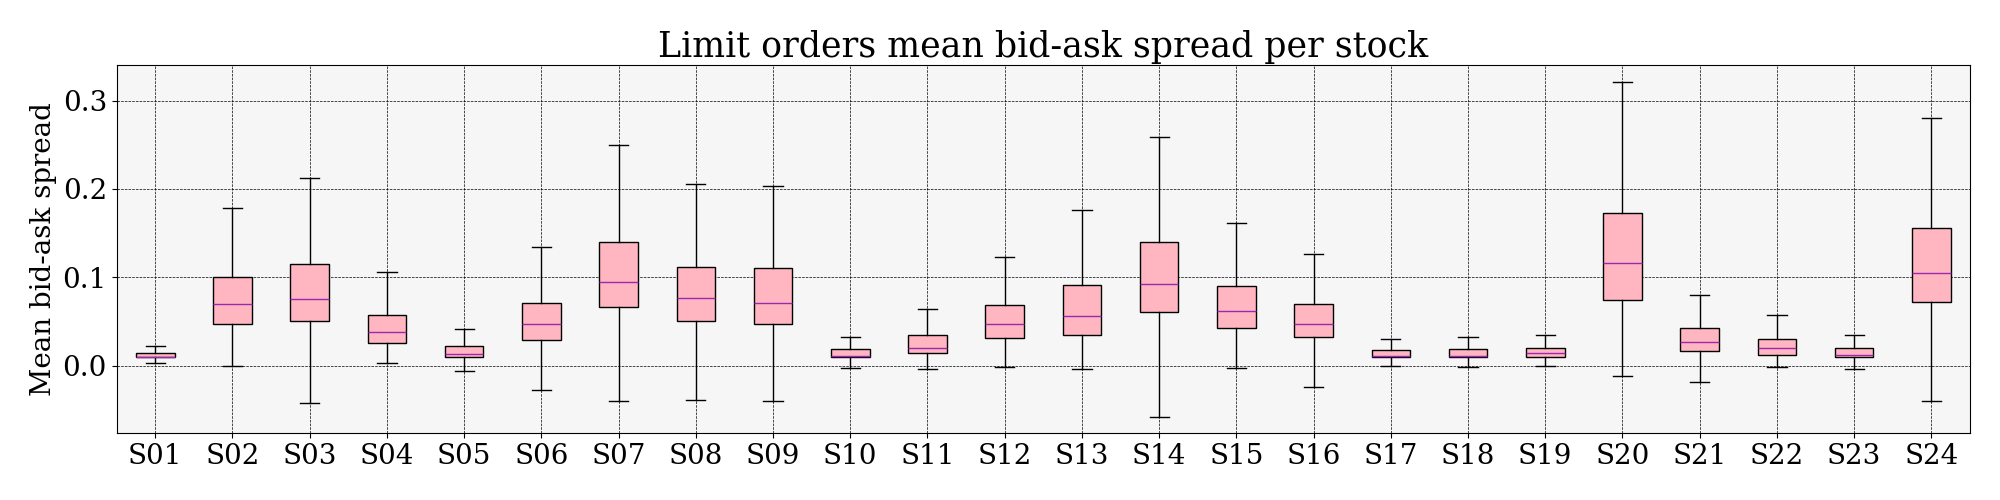
\includegraphics[width=\columnwidth]{figures/mean_spread_per_stock_mo.png}
    \caption{Boxplot of the bid-ask spread for each stock. We only considered the points where a limit order was placed, updated, deleted or traded.}
    \label{fig:spread}
\end{figure}
\begin{multicols}{2}

    \paragraph{Price outliers (number and price value)}
    An \textit{a priori} good feature we derived was the price outliers. First, we considered the number of price outliers for each stock. More precisely, given a stock, we considered all the corresponding observations in the training set, and counted the number of price outliers over the $100$ events.

    We define a price outlier of order $i$ as an order whose price is $i$ ticks away from the best buying or selling price. An illustration of this definition is given on figure \ref{fig:def_outliers}.
    \begin{figure}[H]
        \centering
        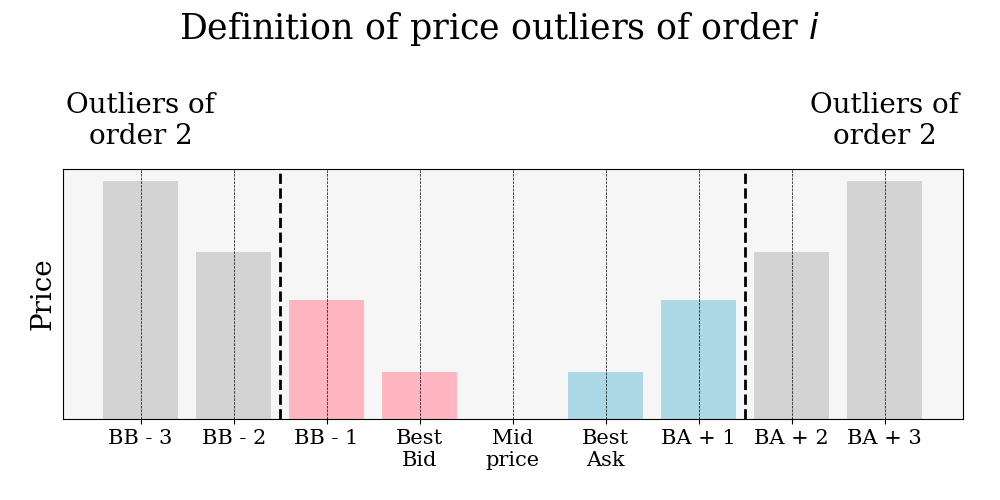
\includegraphics[width=\columnwidth]{figures/price_outliers_def.png}
        \caption{Illustration of the definition of price outliers. In this example, we illustrate the case of a price outlier of order $2$.}
        \label{fig:def_outliers}
    \end{figure}
    While this definition may seem arbitrary since the liquidity and volatility is not the same for all stocks, it is, for our purposes, a fairly sufficient way to set a definition. This is because, the average spread is around $1$ and $10$ ticks for most stocks, and as we can see on figure \ref{fig:nb_outliers}, we already include more than enough outliers for the least liquid stocks (stock 20 for example).

    The second feature we derived was the price value of the outliers. This is done by simply considering, for each stock and corresponding observation, the average price of the outliers over the $100$ events.

    We plot on figure \ref{fig:boxplot_outliers} the boxplot of the number of price outliers for each stock, over all available observations in the training set. We can see that the stocks do not really separate well, and therefore that the number of price outliers does not seem to be a good indicator of the stock. This will be confirmed in the feature importance analysis in the results section.

    On the other hand, we get more interesting results when we look at the value distributions of the price outliers. We plot on figure \ref{fig:boxplot_price_outliers_bid_ask} the boxplot of the bid and ask price outliers for each stock. For example, we can see that stocks 7 and 20, as well as, in a lesser extent, stocks 5, 8, 15, 17, 19 and 23 distinguish themselves from the others by having a higher percentage of outliers. This type of result is what we are looking for, since it gives additional discriminative information about the stocks.

    \paragraph{Price outliers (flux)}
    Similarly, we looked at the flux of the orders that were price outliers. We considered, for each stock and corresponding observation, the average flux of the price outliers over the $100$ events. We did this analysis on $4$ different subsets of the data: ask addition, ask update, bid update and bid addition.
    We plot on figures \ref{fig:flux_ask_add}, \ref{fig:flux_ask_update} and \ref{fig:flux_bid_update} the boxplots corresponding to the first three cases (the bid addition outliers are very similar to the ask addition outliers, so we didn't include them).

    We can see that a variety of stocks are clearly distinguishable. A striking example is stock 20, which stands out alone in the ask addition outliers of order $100$. Therefore, if the test set has a similar distribution, we can expect our model to perform almost perfectly on this stock.

    \paragraph{Other unconclusive features} Among the other features we looked at, we can mention the trade proportion, price and volume per stock, the bid-ask spread distinguished by venue or the proportion of limit orders. None of these features were particularly discriminative.

    \subsection{Preprocessing}

    Building on the previous section, we followed some pre-processing steps before training some models. Depending on the model, we used different pre-processing steps. We will try to describe the most important ones here.

    \subsubsection{Graph models}

    For the graph models, we used the following pre-processing steps:
    \begin{enumerate}
        \item Outliers removal : we removed all observations from the training set for which at least one event had at least one value at more than $7$ standard deviations from the mean. We only considered the price, bid, ask, bid size, ask size and flux features for this operation. This removed $5808$ observations which is around $3.6\%$ of the training set.
        \item Log transformation : we applied a log transformation to the flux, bid size and ask size. This specific transformation preserves the sign of the values :
              $$\tilde{x}= \text{sign}(x)\log(1+|x|)$$
        \item Min-max scaling : we further normalize the bid size and ask size features by applying a min-max scaling to the log-transformed values. The min and max are computed together on both features to preserve their relative scale.
    \end{enumerate}

    While these pre-processing steps are arbitrary, they gave much better results than some standard pre-processing steps such as standard scaling or min-max scaling on the original features.

    \subsubsection{Simple features}

    One set of features that we used for the statistical models and that we can refer to as "simple features" is the following:
    \begin{enumerate}
        \item For each feature present for each event (11 features), compute min, max, mean, median, and standard deviation over the 100 events.
        \item Do the same for the bid-ask spread, the indicator of whether the price is the best bid or ask, and the sum of bid size and ask size.
        \item Add the following features computed over the 100 events:
              \begin{itemize}
                  \item The number of unique order ids.
                  \item The number of orders for each venue.
                  \item The number of each action (new, delete, update).
                  \item The number orders on each side (buy, sell).
                  \item The number of trades.
                  \item The sum of the flux.
              \end{itemize}
    \end{enumerate}
    Once again these features are arbitrary, but they are a good statistical summary of the data, allowing to process a sequence of orders as a single data point in $\R^{89}$.

    \subsection{Graph construction}

    To deal with the temporal and categorical aspects of the data, one idea is to represent the data as a graph that better represents the relationships between the different events. After a bit of trial and error, we made the following arbitrary choices to construct a graph representing a sample :
    \begin{enumerate}
        \item The graph is undirected.
        \item Each event is a node in the graph.
        \item Each venue corresponds to a connex component in the graph.
        \item If two events happen successively at a venue, there is an edge between them.
        \item If two events have the same order id, there is an edge between them.
    \end{enumerate}

    The separation of the graph into connex components corresponding to the venues is motivated by the high frequency nature of the data. Indeed, very few actors can react with high speed to the events happening in another venue, so it makes sense to assume that the events happening in different venues are somewhat independent. Note that the order id is unique to a venue so there should be no edge between the different venues.

    The features that are not encoded in the structure of the graph can be placed on the nodes and the edges.
    \begin{itemize}
        \item Node features: price, bid, ask, bid size, ask size, flux.
        \item Edge features: action, side, trade.
    \end{itemize}
    We also add the venue and a time feature to the nodes, otherwise the model would not be able to distinguish between the different venues, and would not know in which direction the time flows.

        [ADD A FIGURE WITH A GRAPH AND THE CORRESPONDING ORDER BOOK]

    \section{Method}

    In this section, we describe the different models we used. We experimented with three main types of models: recurrent neural networks which are well suited for sequential data, graph neural networks which exploit the graph representation of the data, and statistical models that exploit features extracted from the sequence of events. From the start we knew that our final prediction would be an ensemble of models, so we explored different types of models to maximize the diversity of the ensemble. Indeed the diversity should improve the robustness of the predictions, especially given the change of distribution between the training and the test set.

    \subsection{Recurrent Neural Networks}

    Long-Short Term Memory (LSTM) networks are a type of recurrent neural network that are well suited for sequential data \cite{hochreiter-1997}. We used a simple LSTM model to extract features from the sequence of events. We used the following architecture inspired by the baseline :
    \begin{itemize}
        \item An embedding layer to embed the categorical features (venue, action, side, trade) over $8$ dimensions. The other features are already continuous and do not need to be embedded.
        \item A bidirectional LSTM layer with $128$ hidden units and two layers.
        \item A linear layer with one hidden layer of size $128$.
    \end{itemize}

    This model is simple and fast to train, and it gave us a good baseline to compare with the other models. We quickly reached a validation accuracy of around $50\%$ with this model and some data preprocessing, which was encouraging. However we quickly realized that the model was not robust to the change of distribution between the training and the test set as it only reached around $30\%$ accuracy on the test set.

    \subsection{Graph Attention Networks}

    Graph Attention Networks (GAT) \cite{velickovic-2018} have been shown to be effective in many tasks. Like other graph neural networks, GATs aggregate information from the neighbors of each node to compute its embedding. The main difference with other models is that GATs use an attention mechanism to weight the neighbors of each node. Specifically we used the improved version of GATs suggested in \cite{brody-2021}.

    Let $G$ be an undirected graph with $N$ nodes denoted $\llbracket1, N\rrbracket$. Let $d_1$ be the dimension of the node embeddings, and $h_1,\dots,h_N\in\R^{d_1}$ be the said embeddings. Let $d_2$ be the dimension of the edge embeddings, and $\left\{e_{i,j} \; | 1\leq i,j\leq N\right\}$ be the said embeddings. Let $W_1\in\R^{d'\times d_1}$, $W_2\in\R^{d'\times d_2}$ and $a\in\R^{d'}$. The attention weights are :
    \begin{equation}
        w(h_i,h_j, e_{i,j}) = a^T \leakyrelu(W_1h_i + W_1h_j + W_2e_{i,j})
    \end{equation}
    The attention weights are normalized using the softmax operator :
    \begin{equation}
        \alpha_{ij} = \frac{\exp(w(h_i,h_j, e_{i,j}))}{\sum_{k\in\mathcal{N}_i}\exp(w(h_i,h_k, e_{i,k}))}
    \end{equation}
    where $\mathcal{N}_i$ denotes the set of neighbors of node $i$ in $G$. The embedding of node $i$ is then computed as :
    \begin{equation}
        h_i' = \leakyrelu\left(\sum_{j\in\mathcal{N}_i}\alpha_{ij}W_1h_j\right)
    \end{equation}
    In general we will use multi-head attention, with $K$ heads, $a^{(1)},\dots,a^{(K)}\in\R^{d'/K}$, $W_1^{(1)},\dots,W_1^{(K)}\in\R^{d'/K\times d_1}$ and $W_2^{(1)},\dots,W_2^{(K)}\in\R^{d'/K\times d_2}$ :
    \begin{equation}
        h_i' = \leakyrelu\left(\frac{1}{K}\sum_{k=1}^K\sum_{j\in\mathcal{N}_i}\alpha_{ij}^{(k)}W_1^{(k)}h_j\right)
    \end{equation}
    Furthermore, we will stack multiple GAT layers to obtain a deeper model. We may also apply a multi-layer perceptron to the embeddings of the last layer to obtain a more expressive representation. This model is easily parallelizable which is useful for mini-batch training.

    \subsection{Other graph models}

    We started out with GAT models because we already had some experience with them, and they were very effective. However, we also trained other graph models to diversify our ensemble (as long as they supported edge features in the graph). Here is an exhaustive list of models that gave us acceptable results and were added to the ensemble (in no particular order) :
    \begin{itemize}
        \item Generalized GNN \cite{li-2020}
        \item Pathfinder Discovery Network \cite{rozemberczki-2021}
        \item Principal Neighbourhood Aggregation \cite{corso-2020}
        \item Graph transformer \cite{shi-2020}
        \item General GNN \cite{you-2020}
    \end{itemize}

    None of these models performed as well as the GAT models (although this may be due to more superficial hyperparameter tuning), but they did improve the diversity of the ensemble.

    \subsection{Statistical models}

    We used multiple statistical models on simple features extracted from the data to diversify our ensemble. These models are intuitively more robust because they rely on simple features that are less likely to be affected by the change of distribution. Here is a non exhaustive list of the models we used :
    \begin{itemize}
        \item Random Forest Classifier
        \item Ada Boost Classifier
        \item Logistic Regression
        \item K-Nearest Neighbors
        \item Ridge Classifier
    \end{itemize}

    \subsection{Franck Zibi's model}

    Last year's CFM challenge also involved adapting to a change of distribution between the training and the test set. Inspired by the winning solution of last year's challenge, we devised a similar model. It is a simple model motivated by boosting methods, that learns the residuals of the predictions of a base model.
    \begin{enumerate}
        \item A random forest classifier is trained on the training set. This model is able to output a probability distribution over the classes.
        \item For each class, three models are trained to predict the residuals of the random forest classifier (a random forest regressor, a k-nearest neighbors regressor and a linear regressor).
        \item For each class, the three models are stacked using a linear regressor.
    \end{enumerate}

    We can then simply predict the class of a sample by adding the output of the random forest classifier to the output of the stacked models, and taking the class with the highest probability.

    \subsection{Ensemble}

    \section{Training}

    For all the models we used the same split of the training set into a training and a validation set. We used $90\%$ of the training set for training and $10\%$ for validation. We did not use cross validation because the training set was already very large and well-balanced.

    \subsection{Loss}
    Like in most classification tasks, we used the cross-entropy loss to train our models. When it became clear that the distribution of the test set was very different from the training set, we experimented with different loss functions to make the models more robust to this change. We settled on Minimum Class Confusion (MCC) loss \cite{jin-2020} which aims at minimizing the confusion between the classes on a target domain (the test set in our case).

    Let $(X_n)_{1\leq n\leq N}$ be a batch of testing samples, and $\hat{Y}_n = F(X_n)\in\R^{24}$ be the output of the model for sample $X_n$. MCC uses temperature scaling to soften the predictions :
    \begin{equation}
        \tilde{Y}_{n,i} = \frac{\exp\left(\hat{Y}_{n,i}/T\right)}{\sum_{j=1}^{24}\exp\left(\hat{Y}_{n,j}/T\right)}
    \end{equation}
    where $T>0$ is the temperature (we used $T=2.5$). We then compute an entropy over the predictions :
    \begin{equation}
        H_n = -\sum_{i=1}^{24}\tilde{Y}_{n,i}\log\left(\tilde{Y}_{n,i}\right)
    \end{equation}
    This entropy will be used to give more importance to samples for which the model is more confident. We then use the following weights :
    \begin{equation}
        W_n = N\times\frac{1+\exp(-H_n)}{\sum_{i=1}^{N} 1+\exp(-H_i)}
    \end{equation}
    where $N$ is the batch size. This weight makes use of Laplace smoothing for numerical stability. Finally the class confusion between class $i$ and class $j$ is given by :
    \begin{equation}
        C_{i,j} = \tilde{Y}_{\cdot,i}^T \text{diag}(W_1,\dots,W_B) \tilde{Y}_{\cdot,j}
    \end{equation}
    This class confusion is normalized to account for class imbalance :
    \begin{equation}
        \tilde{C}_{i,j} = \frac{C_{i,j}}{\sum_{k=1}^{24}C_{i,k}}
    \end{equation}
    Which gives us the final loss :
    \begin{equation}
        \mathcal{L}_{\text{MCC}} = \frac{1}{24}\sum_{i=1}^{24}\sum_{j=1}^{24}\left|\tilde{C}_{i,j}\right|
    \end{equation}

    Note that this note does not use labels from the target domain, and is therefore unsupervised. It can simply be added to the supervised loss to make the model more robust to the change of distribution :
    \begin{equation}
        \mathcal{L} = \mathcal{L}_{\text{CE}} + \mu\mathcal{L}_{\text{MCC}}
    \end{equation}
    we found that $\mu=0.1$ was a good value and we could easily go as high as $\mu=1$ or $\mu=10$ for models that trained easily. In practice this MCC loss is computed on a batch of the test set every $10$ iterations of the training loop. We found that it did raise the accuracy of the models on the test set by around $5\%$.

    \subsection{Optimizer}

    We used the Adam optimizer with a starting learning rate of $5\times10^{-3}$. We did not use weight decay as it hindered the training of the models.

    We used a scheduler to automatically decrease the learning rate. The scheduler decreased the learning rate by a factor of $0.95$ every epoch, which yielded a learning rate of around $1\times10^{-3}$ after $30$ epochs which is a typical number of epochs for our models.

    \begin{figure}[H]
        \centering
        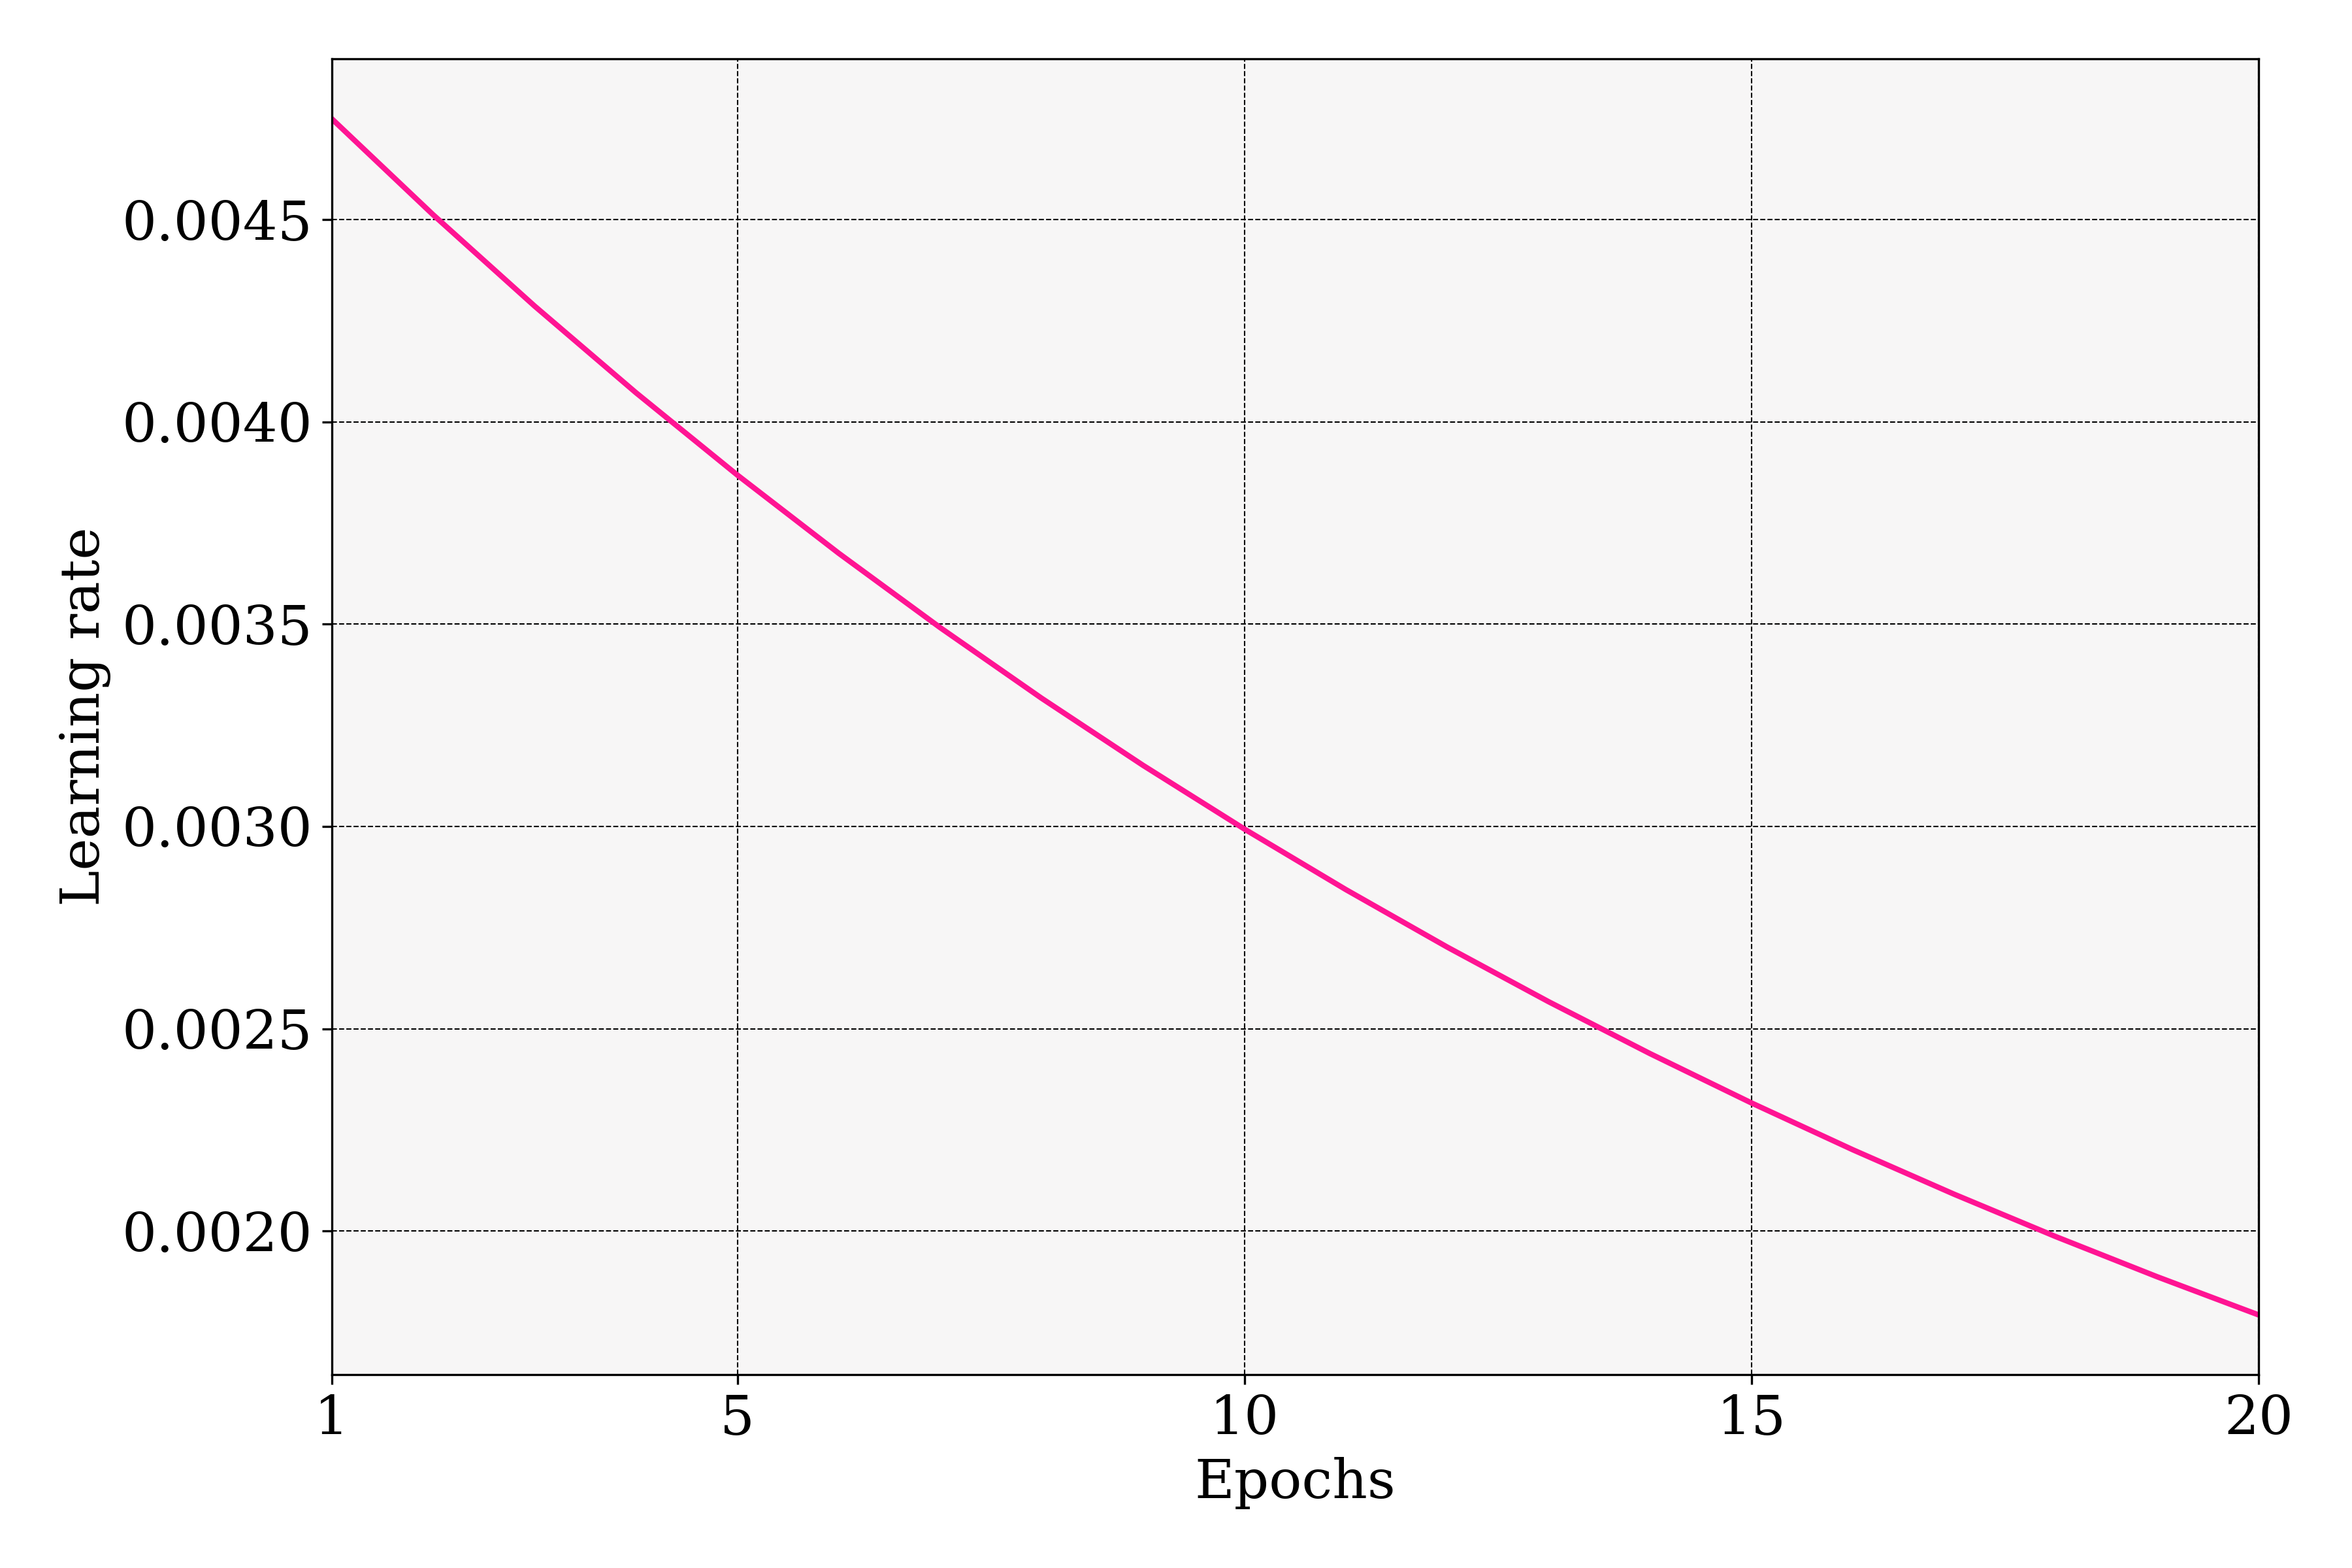
\includegraphics[width=\columnwidth]{figures/learning_rate.png}
        \caption{Learning rate schedule.}
        \label{fig:learning_rate}
    \end{figure}

    We generally stopped the training quickly when the accuracy on the validation set stopped increasing significantly. This is motivated by the change of distribution between the training and the test set, which means that we do not want to overfit the training set.

    \subsection{Other unsuccessful experiments}

    We tried other tricks to make the models more robust to the change of distribution.
    \begin{itemize}
        \item We experimented with data augmentation on the training set : given the high stochasticity of the data, we could easily generate new samples by adding some noise to the prices, the volumes, the flux, etc.
        \item Starting with a trained model, we extracted the test samples for which it was the most confident, and submitted them to the leaderboard (with the rest left at random). We could infer that we had around $80\%$ accuracy on these samples. Thus we tried fine-tuning a model on these samples, but it did not improve the accuracy on the test set.
    \end{itemize}

    \subsection{Monitoring metrics}

    For intellegible training and comparison of deep learning models, we monitored the following metrics at each epoch :
    \begin{itemize}
        \item Training accuracy (figure \ref{fig:train_accuracy})
        \item Validation accuracy (figure \ref{fig:val_accuracy})
        \item Training loss (figure \ref{fig:train_loss})
        \item Validation loss (figure \ref{fig:val_loss})
        \item MCC loss on the test set (figure \ref{fig:mcc_loss})
    \end{itemize}

    These metrics allowed us to quickly stop the training when the model stopped improving, and to compare the different models. As in most classification tasks, the validation accuracy was the most important metric. Considering we used the same cross-entropy loss for all the models, the loss function can provide additional insight into the confidence of the model in the predictions.

    \begin{figure}[H]
        \centering
        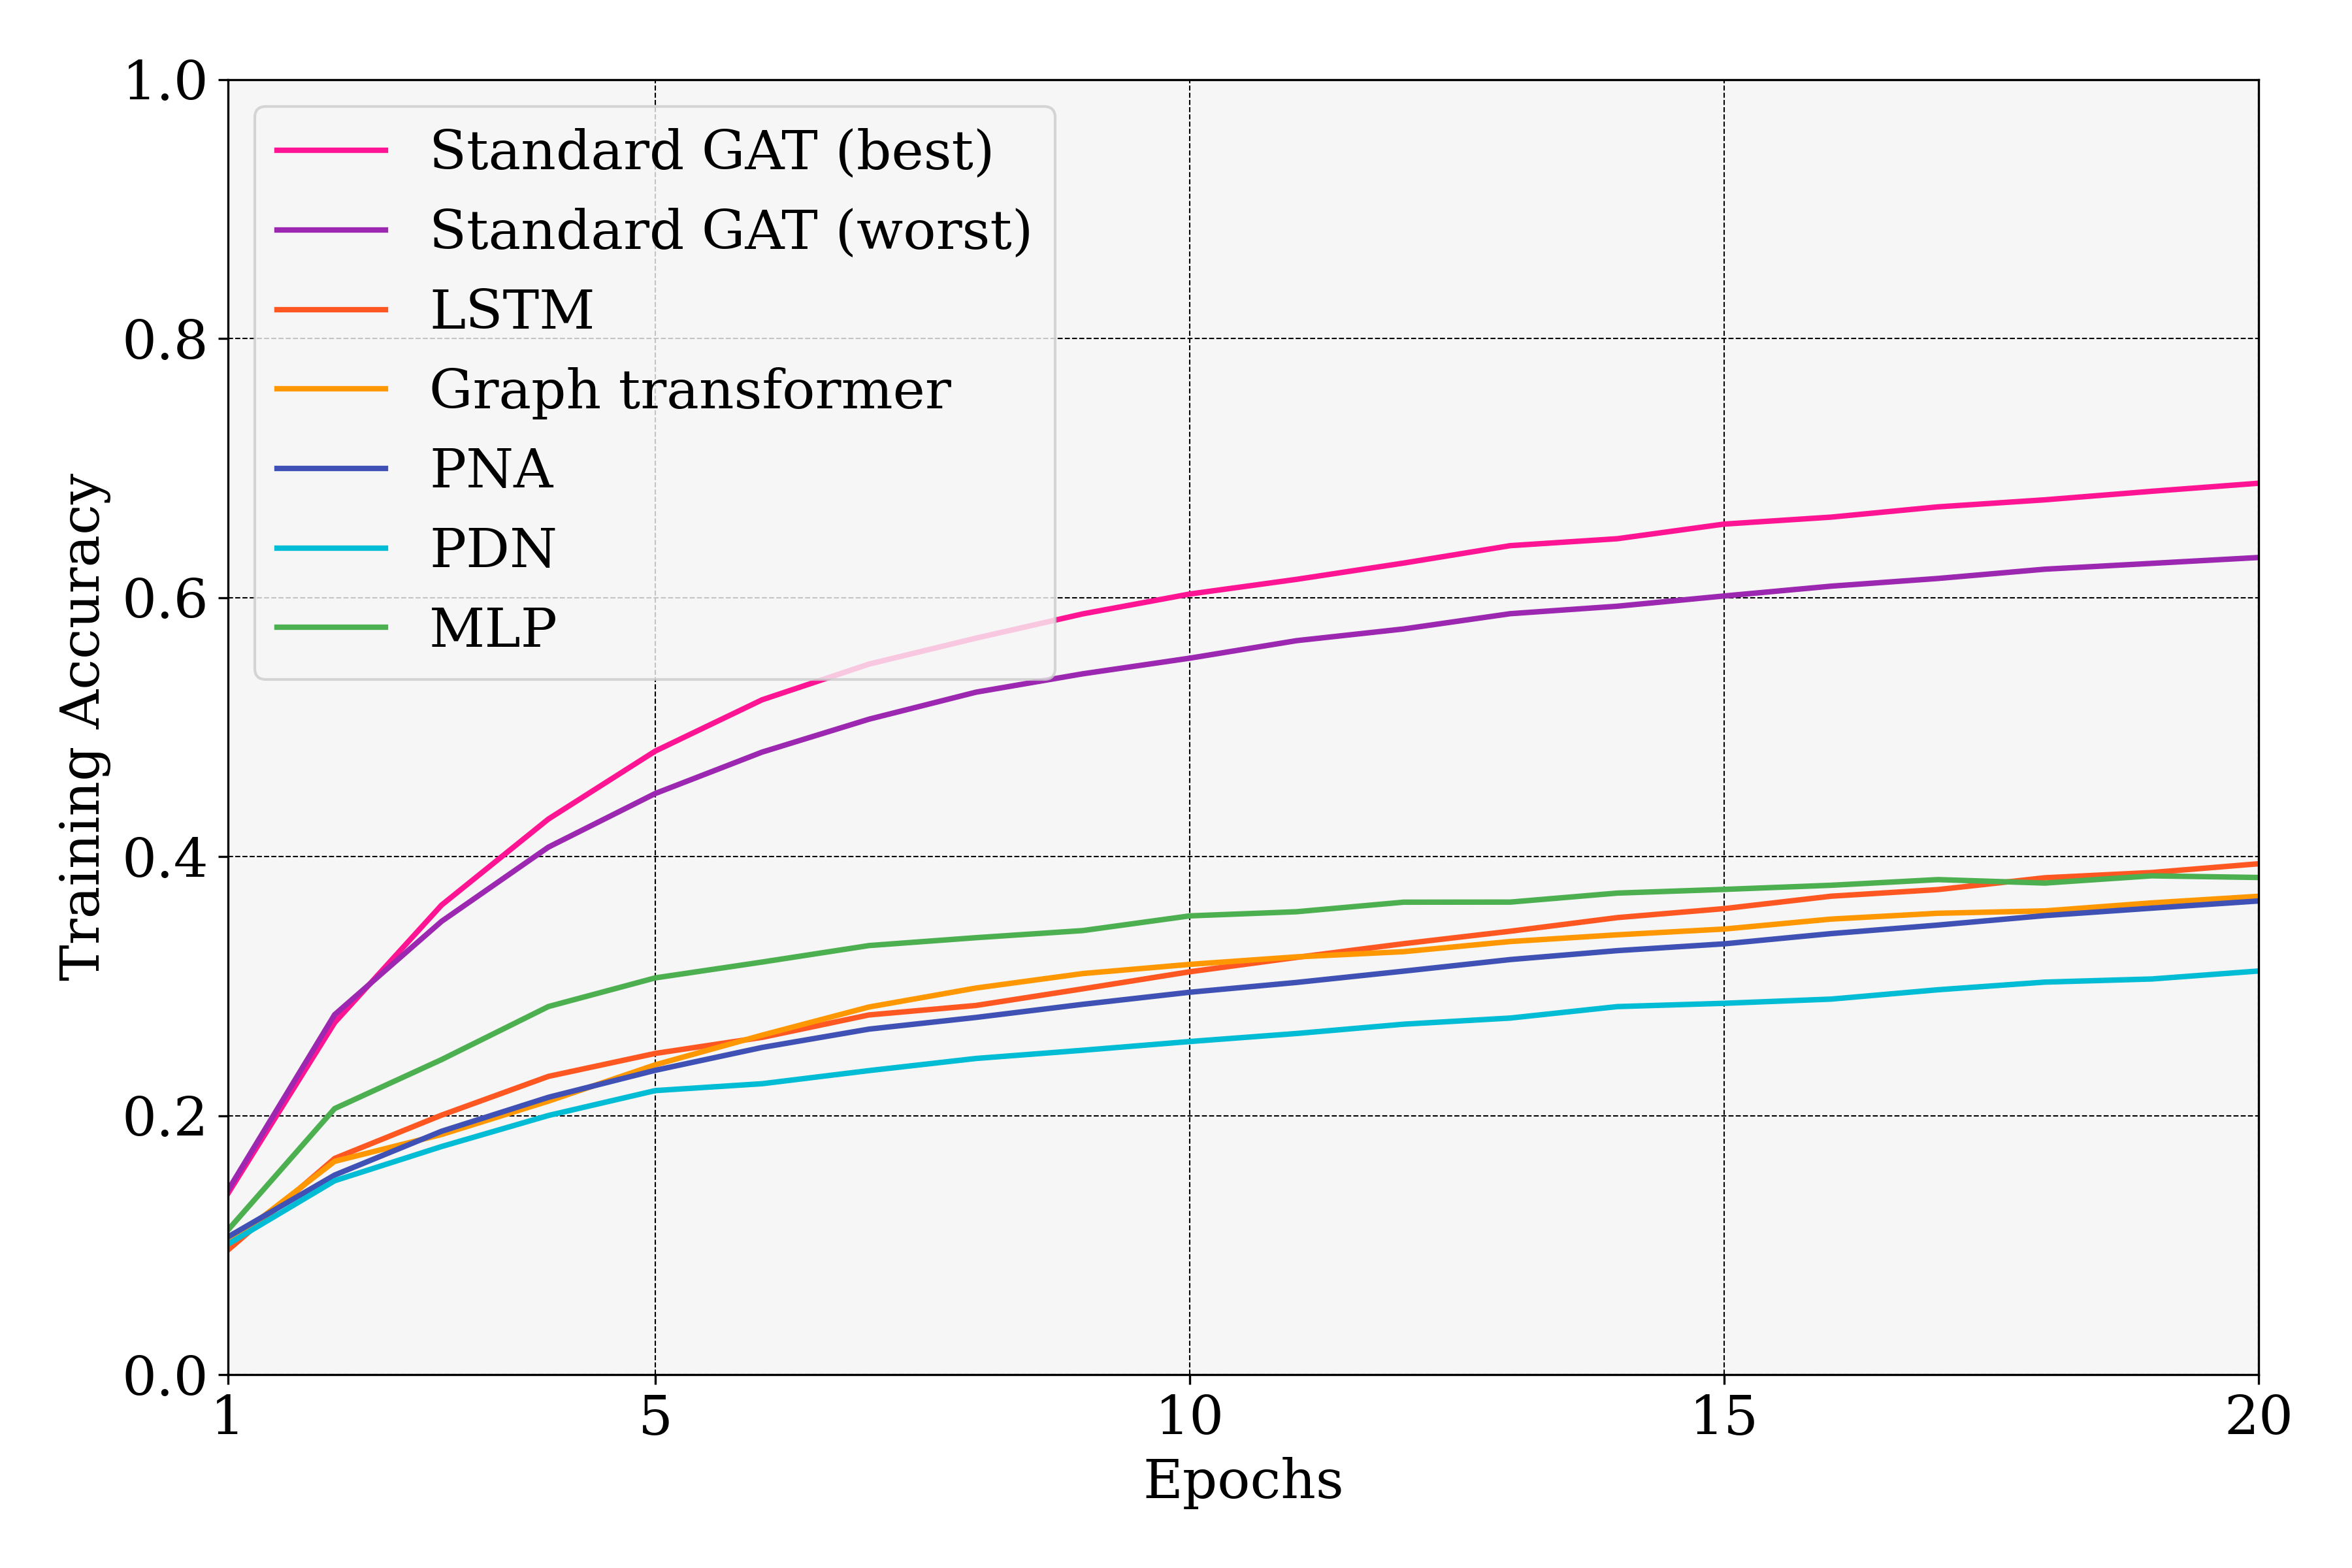
\includegraphics[width=\columnwidth]{figures/train_accuracy.png}
        \caption{Training accuracy}
        \label{fig:train_accuracy}
    \end{figure}

    Figures \ref{fig:train_accuracy} and \ref{fig:val_accuracy} provide multiple insights. First, we can see that the models are not overfitting the training set, as the training and validation accuracy are extremely close. Second, the training procedure is stable, and the models converge quickly, at least for the GAT models. The other models (LSTM, Graph transformer, PNA, PDN, MLP) might benefit from a different optimizer, but we did not have the time to experiment with this. Finally, we note that the GAT models largely outperform the other models, which is why we used them as the main models in our ensemble. The two GAT models presented are the worst one and the best one from the ensemble.

    \begin{figure}[H]
        \centering
        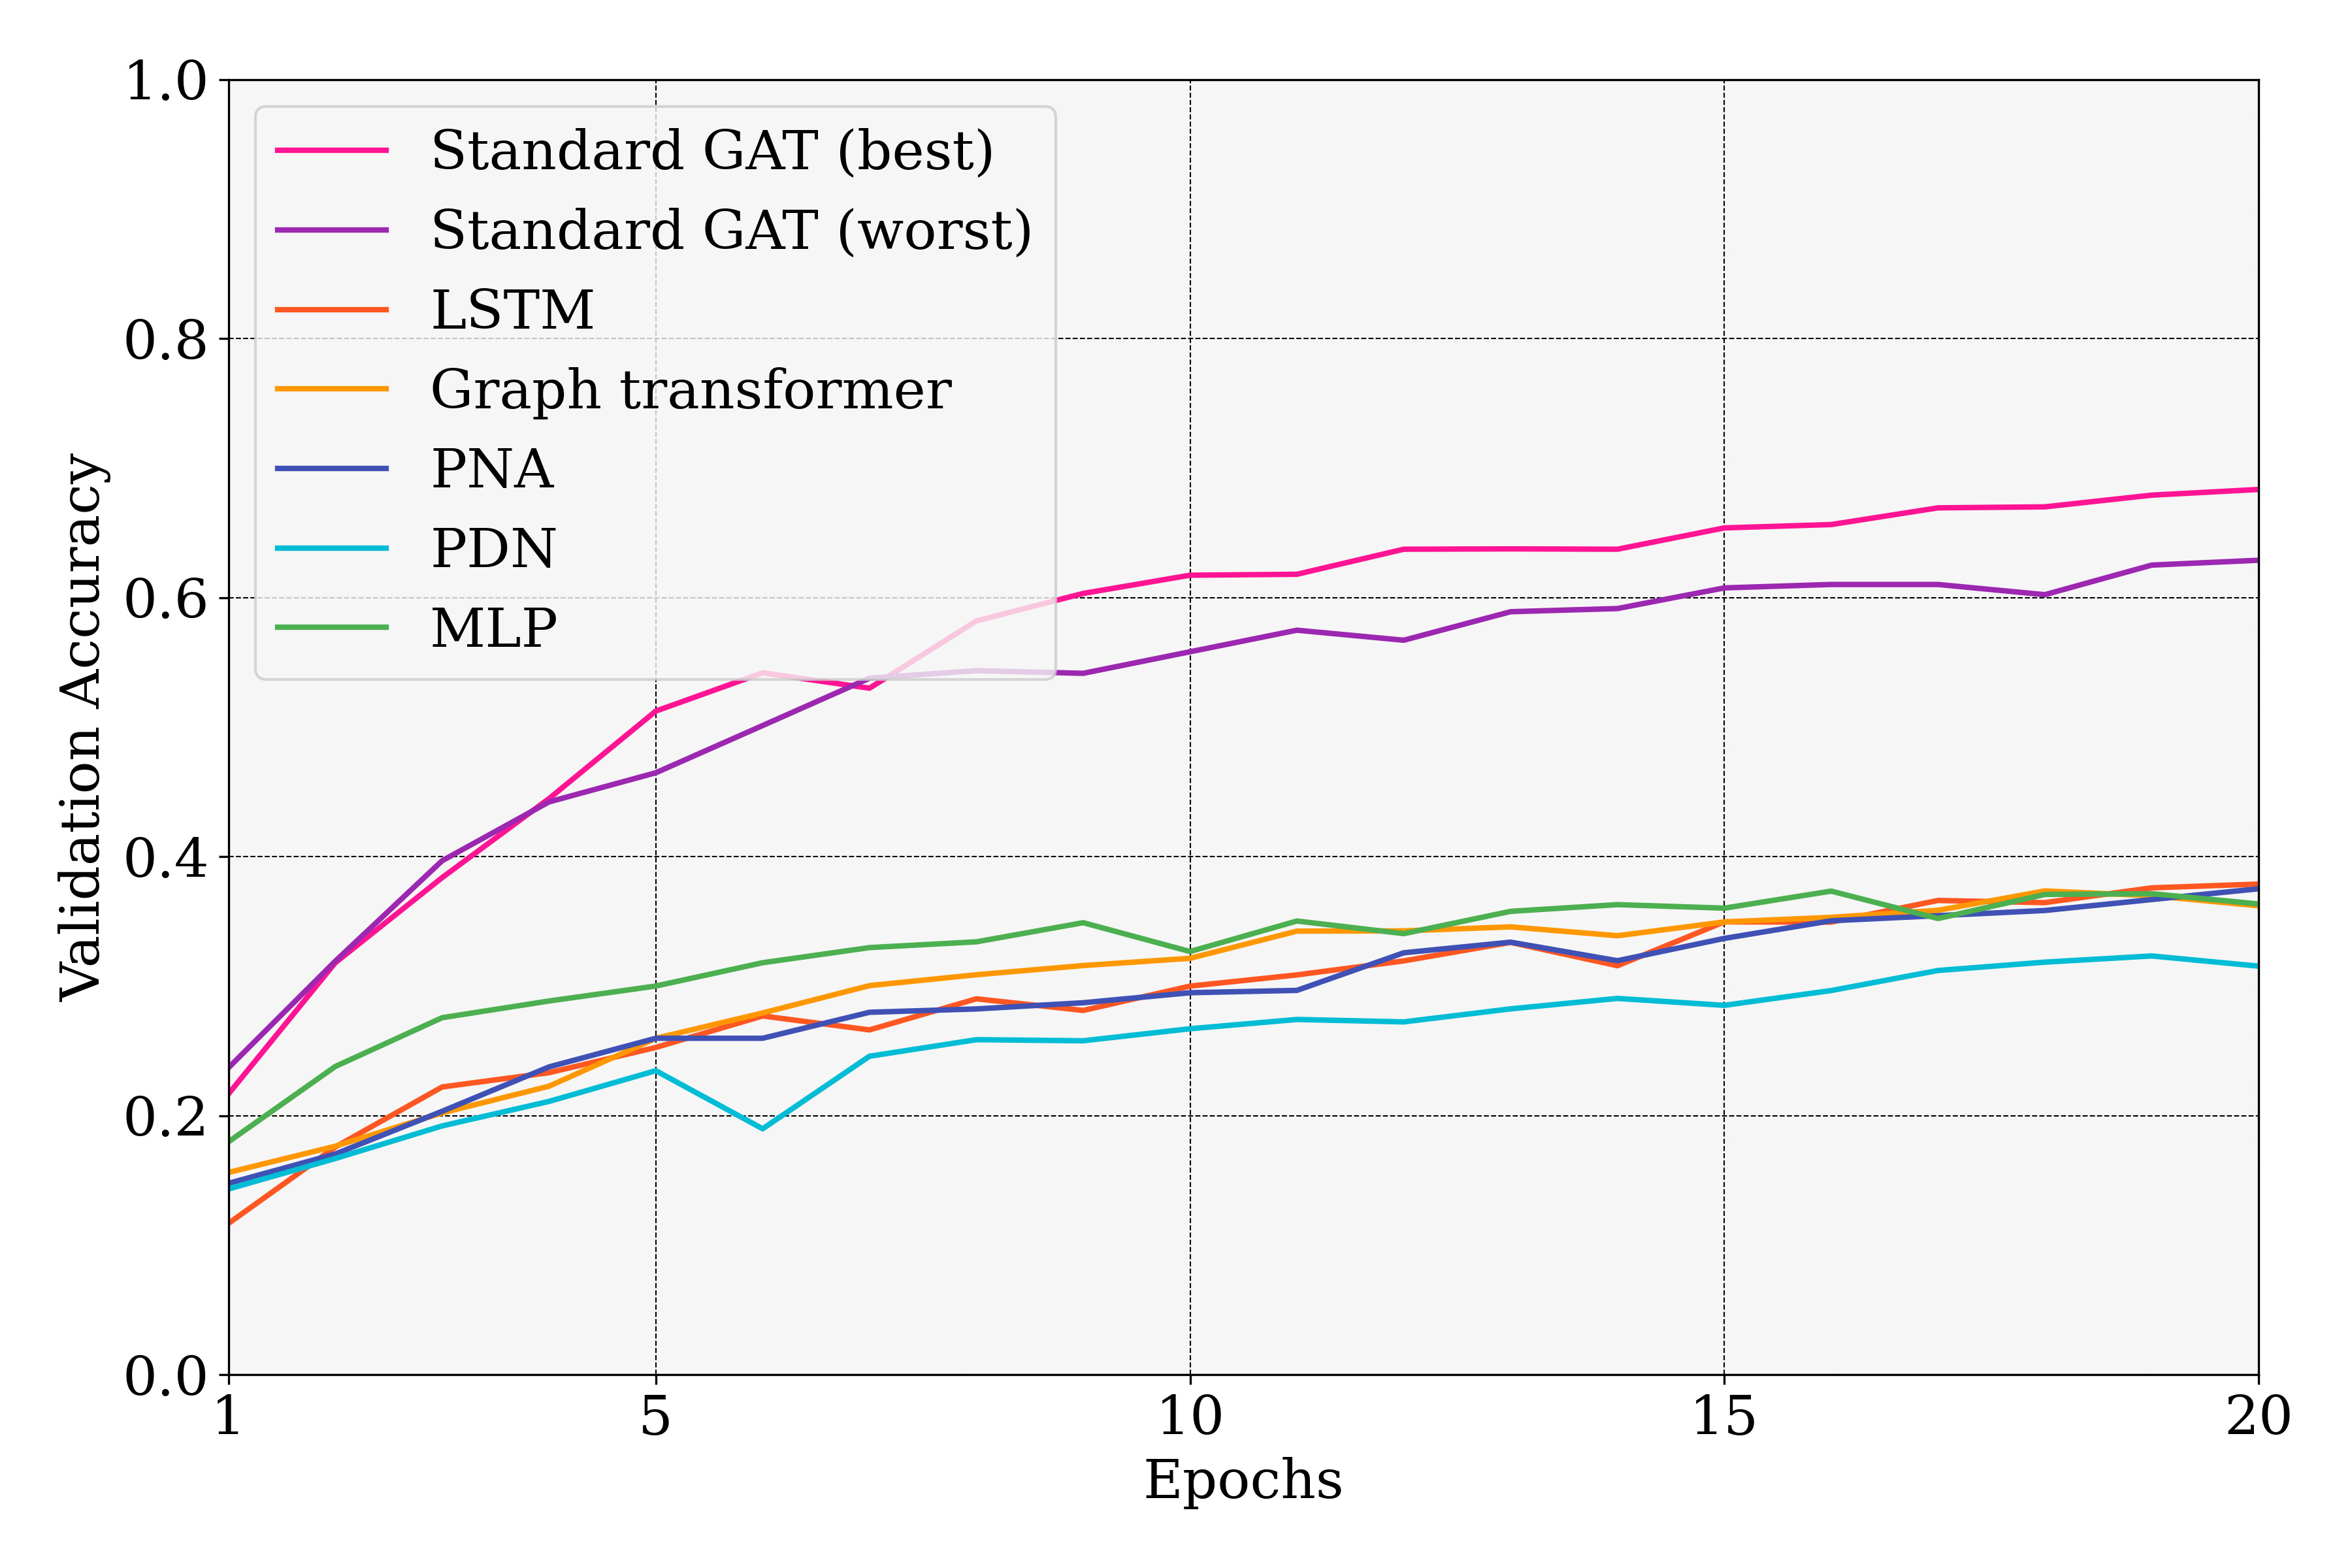
\includegraphics[width=\columnwidth]{figures/val_accuracy.png}
        \caption{Validation accuracy}
        \label{fig:val_accuracy}
    \end{figure}

    \section{Results}
    We present our main accuracy results in table \ref{tab:results}. The very first thing we note is the low accuracies on the test set. As we mentioned earlier, the distribution of the test set is very different from the training set, and this is reflected in the low accuracies. This leads to vastly different models on the validation set getting similar accuracies on the test set.

    The GAT model gives the best results with validation accuracies greater than $70\%$. However it also fails to generalize to the test set. Note that the Generalized GNN model has good results but its training was not stable, so we would not trust it as much as the GAT models. The models based on features (Franck Zibi's and the MLP one) have some of the worst results, which is disappointing since we expected them to be more robust to the change of distribution.

    Finally the ensemble of all the models gives us the best results with a test accuracy of $40\%$. We expected the ensemble to give us the best results, but we were surprised by the low accuracy, as it only gives us a $5\%$ improvement over the best single model.

    \begin{table}[H]
        \begin{center}
            \resizebox{\columnwidth}{!}{
                \begin{tabular}{|c|c|c|c|}
                    \hline
                    \textbf{Model description} & \textbf{Training acc.} & \textbf{Validation acc.} & \textbf{Test acc.} \\
                    \hline
                    PDN                        & 0.42                   & 0.43                     & 0.23               \\
                    \hline
                    MLP                        & 0.42                   & 0.41                     & 0.24               \\
                    \hline
                    Franck Zibi's model        & 0.95                   & 0.42                     & 0.25               \\
                    \hline
                    Graph transformer          & 0.44                   & 0.43                     & 0.29               \\
                    \hline
                    General GNN                & 0.43                   & 0.42                     & 0.30               \\
                    \hline
                    PNA                        & 0.47                   & 0.45                     & 0.30               \\
                    \hline
                    LSTM                       & 0.57                   & 0.44                     & 0.30               \\
                    \hline
                    GAT (50 epochs)            & 0.75                   & 0.71                     & 0.33               \\
                    \hline
                    GAT (20 epochs)            & 0.72                   & 0.68                     & 0.34               \\
                    \hline
                    Generalized GNN            & 0.73                   & 0.71                     & 0.35               \\
                    \hline
                    Final ensemble             &                        &                          & 0.40               \\
                    \hline
                \end{tabular}
            }
        \end{center}
        \caption{Main accuracy results}
        \label{tab:results}
    \end{table}


    \subsection{Statistical models}
    \paragraph{Random Forest Classifier}
    Throughout our experiments, we found the random forest classifier handy for feature selection, as well as for training a model purely based on hand-crafted features.

    We present in this section the results of $2$ random forest classifiers that we trained. The first model was trained on the Bid-Ask spread, the Bid and Ask volume, the number of price outliers, the price outliers, the flux of the price outliers, and the proportion of each venues on which the orders were placed. The second model was only trained on a subset of the features of the first model, which were the Bid-Ask spread, the Bid and Ask volume and the venue proportion.

    We obtained a very important result that framed our approach for the rest of the challenge. We found that the first model had a $49\%$ accuracy on the validation set, while the second model had a $28\%$ accuracy. However, both models performed very similarly on the test set, with an accuracy of respectively $22\%$ and $20\%$. This result is very important because it gives us a clear indication that the "outlier" features, while being very discriminative on the training set, are almost irrelevant on the test set. At this point, we had $2$ choices: either we could eliminate the outlier features from our ensemble, or we could try to find a model that would be able to detect how the "outlier" features distribution changed in the test set.

    \subsection{Predictions analysis}

    \section{Conclusion}

    \newpage
    \bibliography{bibliography}

\end{multicols}

\newpage
\appendix
% \vspace{5mm}
\begin{center}
    {\Large \bfseries Appendix} \\
\end{center}
\begin{figure}[H]
    \centering
    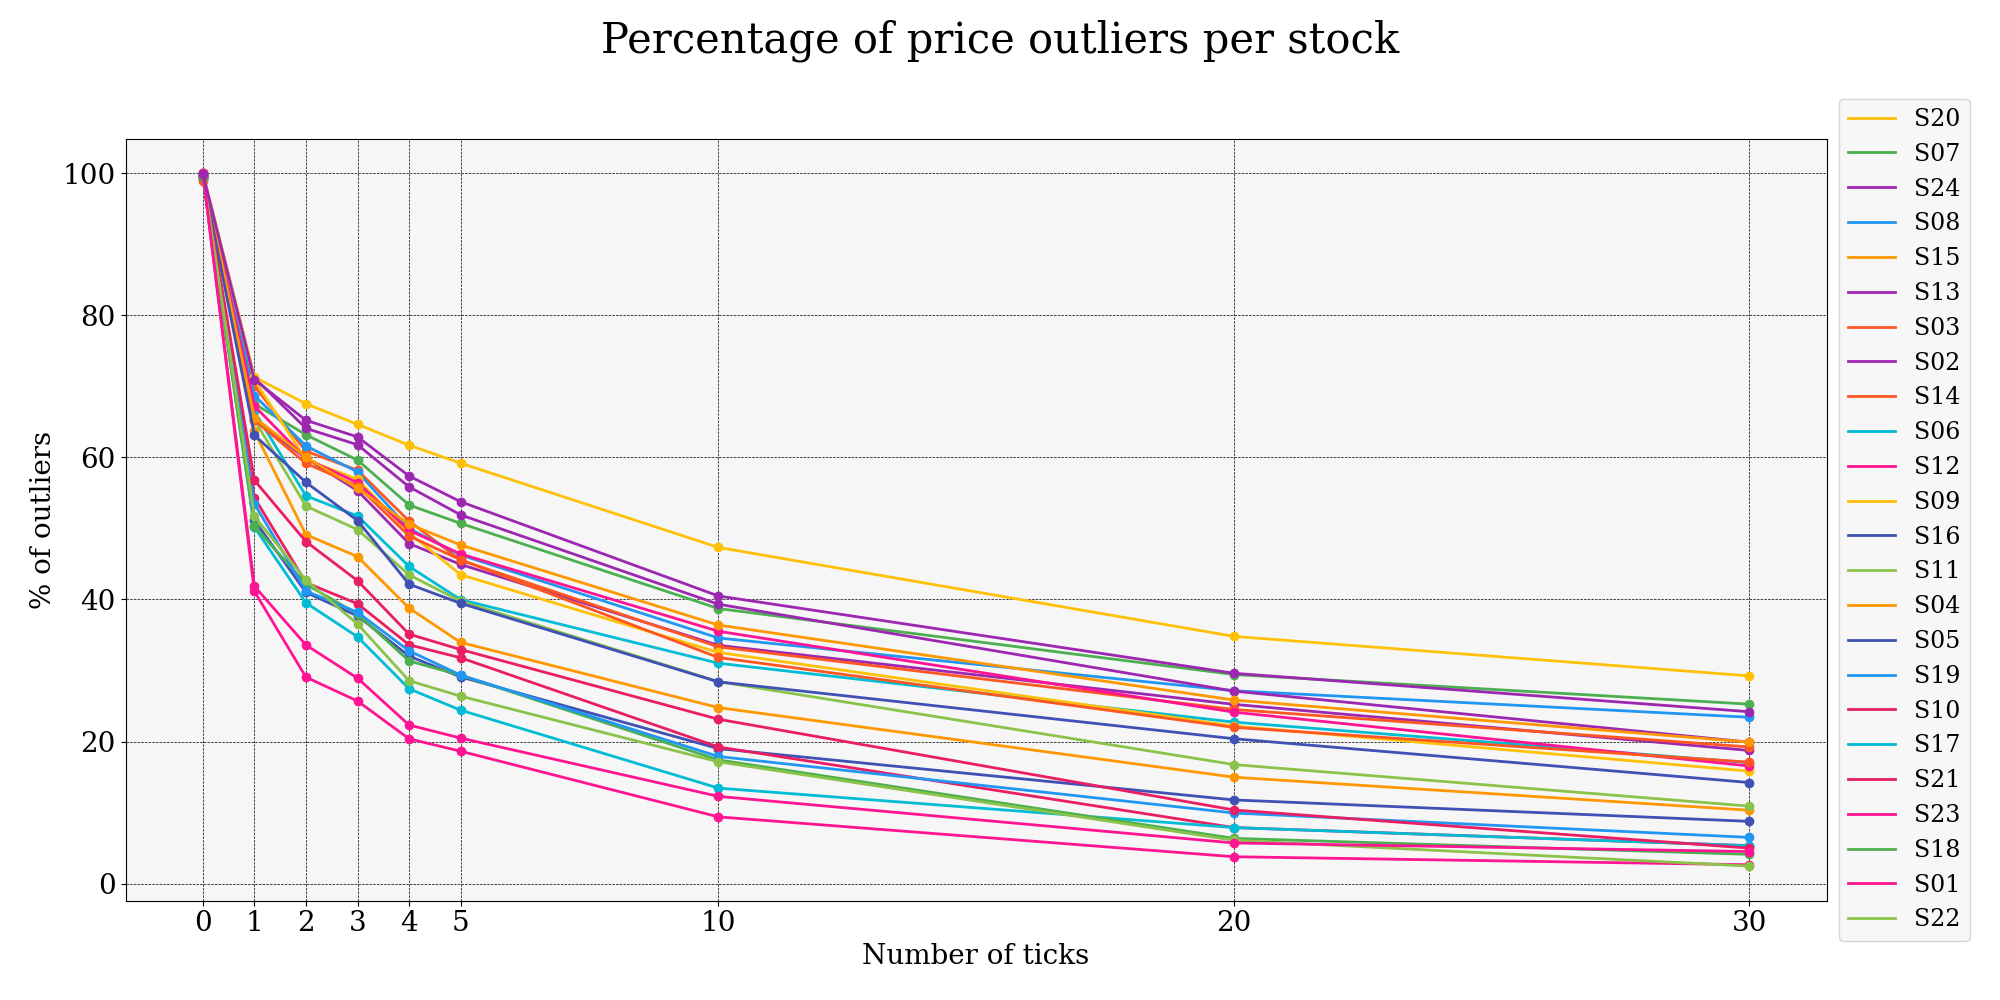
\includegraphics[width=\columnwidth]{figures/percentage_outliers_per_stock.png}
    \caption{Percentage of price outliers per number of ticks.}
    \label{fig:nb_outliers}
\end{figure}

\begin{figure}[H]
    \centering
    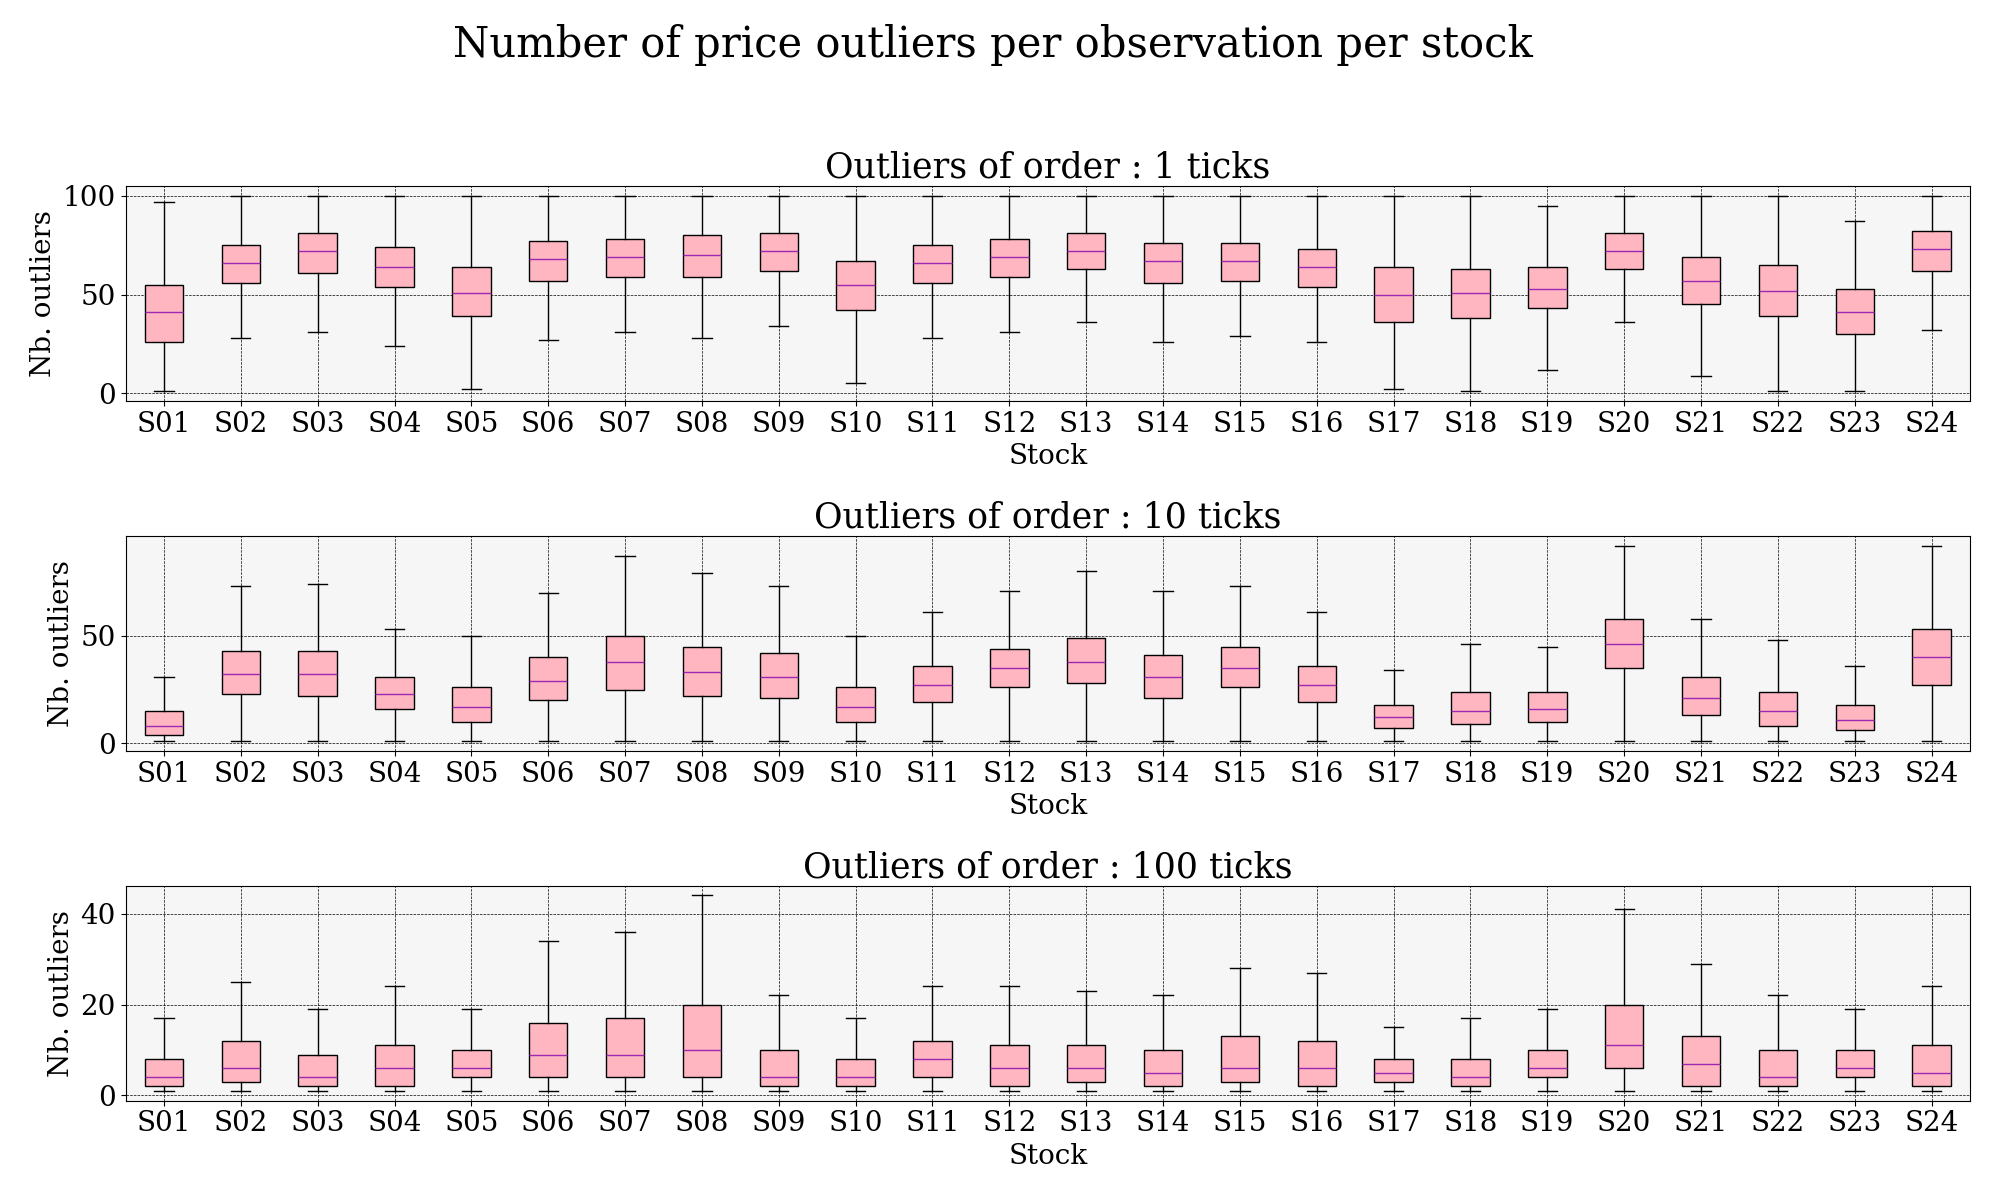
\includegraphics[width=\columnwidth]{figures/boxplot_nb_outliers.png}
    \caption{Boxplot of the number of price outliers for each stock.}
    \label{fig:boxplot_outliers}
\end{figure}

\begin{figure}[H]
    \centering
    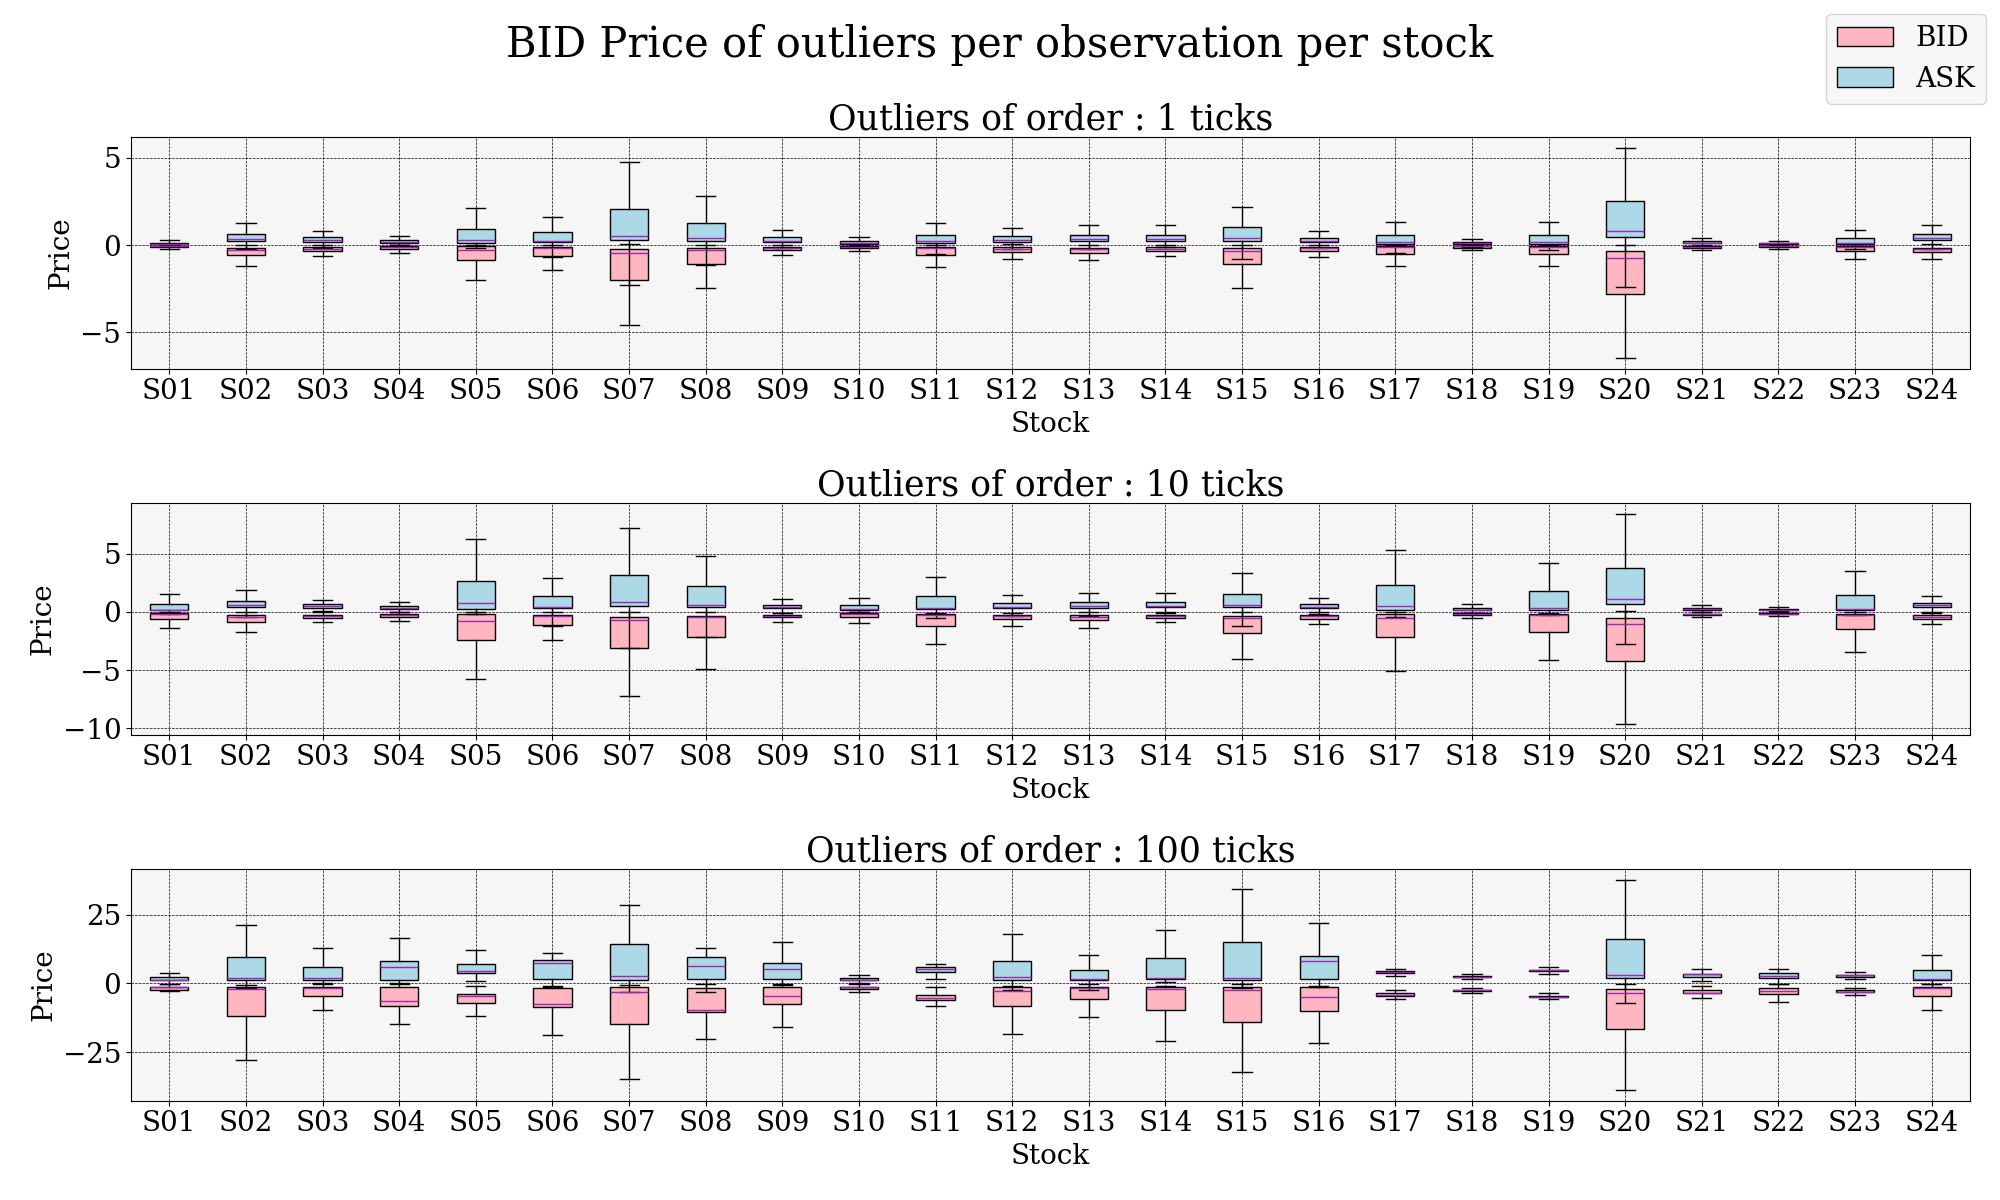
\includegraphics[width=\columnwidth]{figures/boxplot_price_outliers_BID_ASK.png}
    \caption{Boxplot of the bid and ask price outliers for each stock.}
    \label{fig:boxplot_price_outliers_bid_ask}
\end{figure}

\begin{figure}[H]
    \centering
    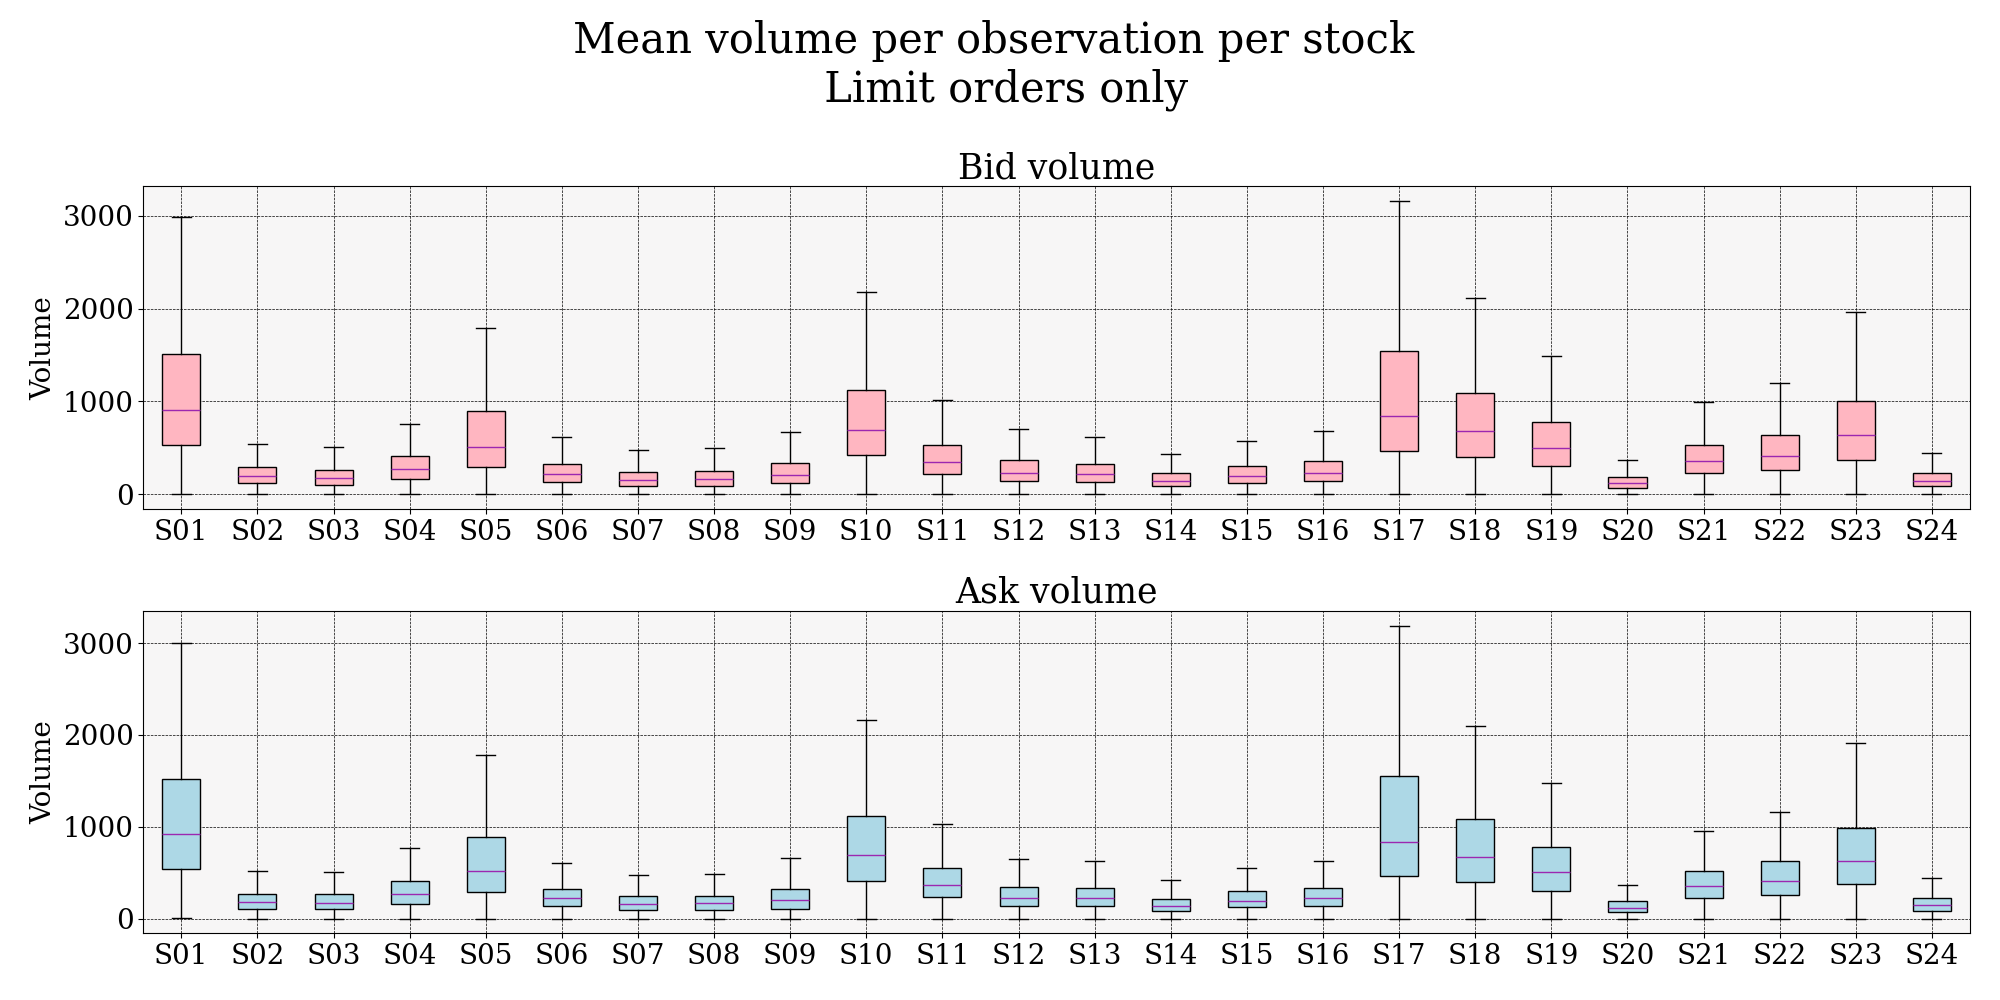
\includegraphics[width=\columnwidth]{figures/boxplot_volume_per_stock.png}
    \caption{Boxplot of the bid and ask volume for each stock.}
    \label{fig:volume}
\end{figure}

\begin{figure}[H]
    \centering
    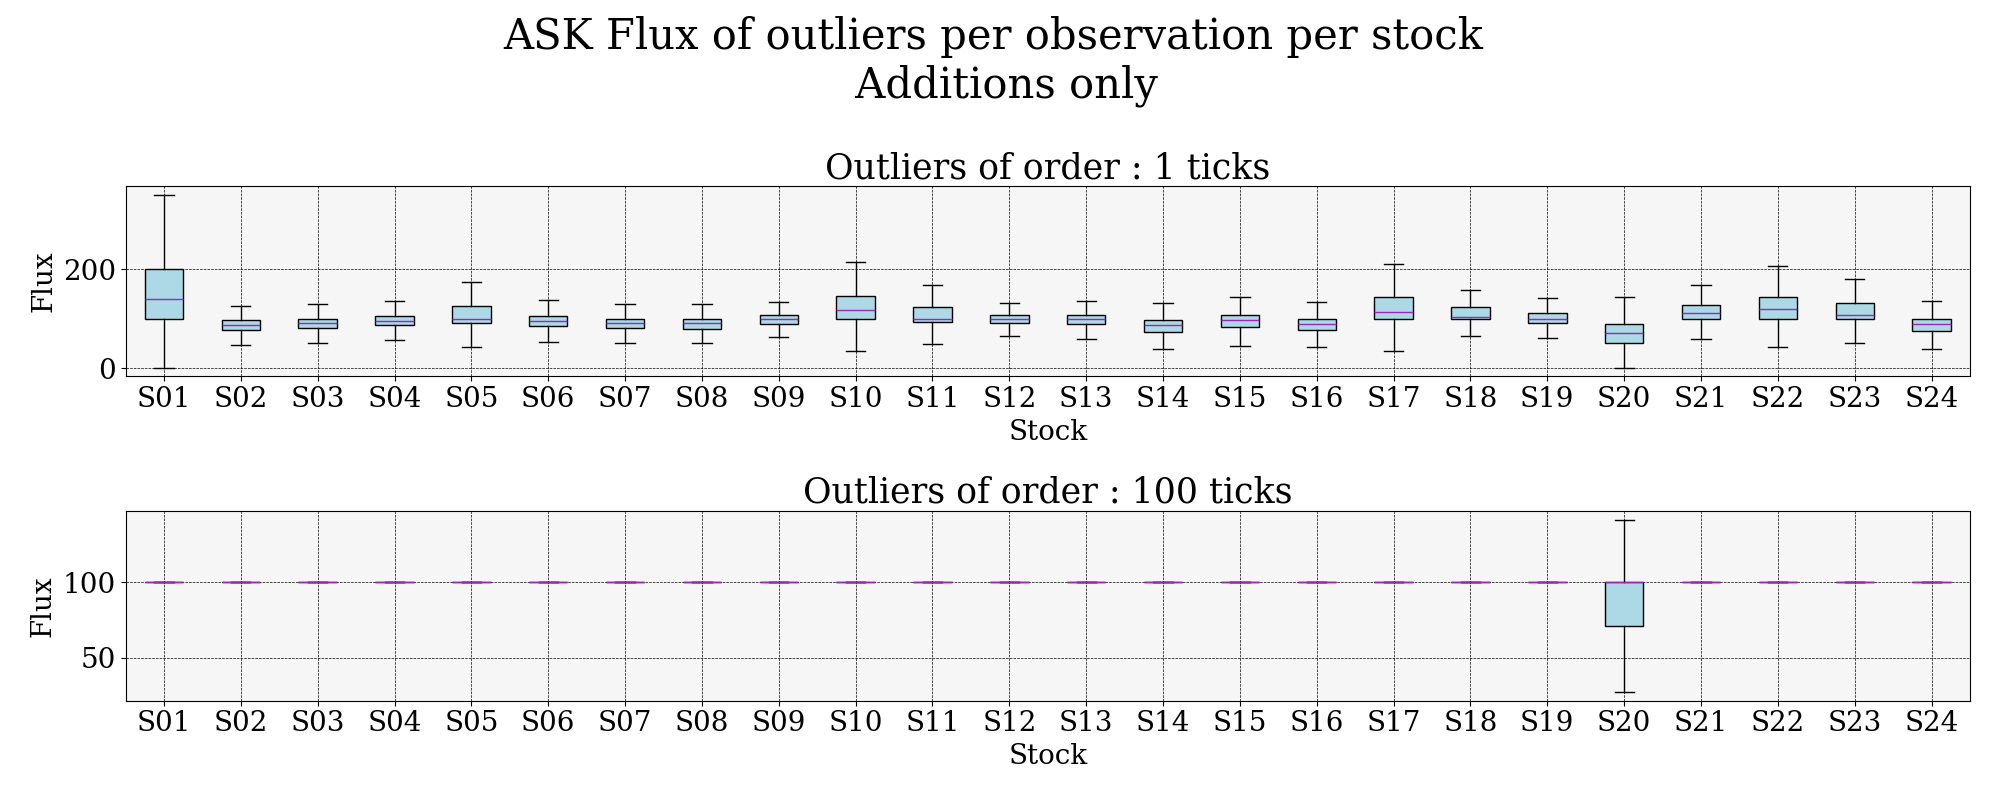
\includegraphics[width=\columnwidth]{figures/boxplot_flux_outliers_ASK.png}
    \caption{Boxplot of the flux of the ask price outliers for each stock. Only the ask addition outliers are considered.}
    \label{fig:flux_ask_add}
\end{figure}

\begin{figure}[H]
    \centering
    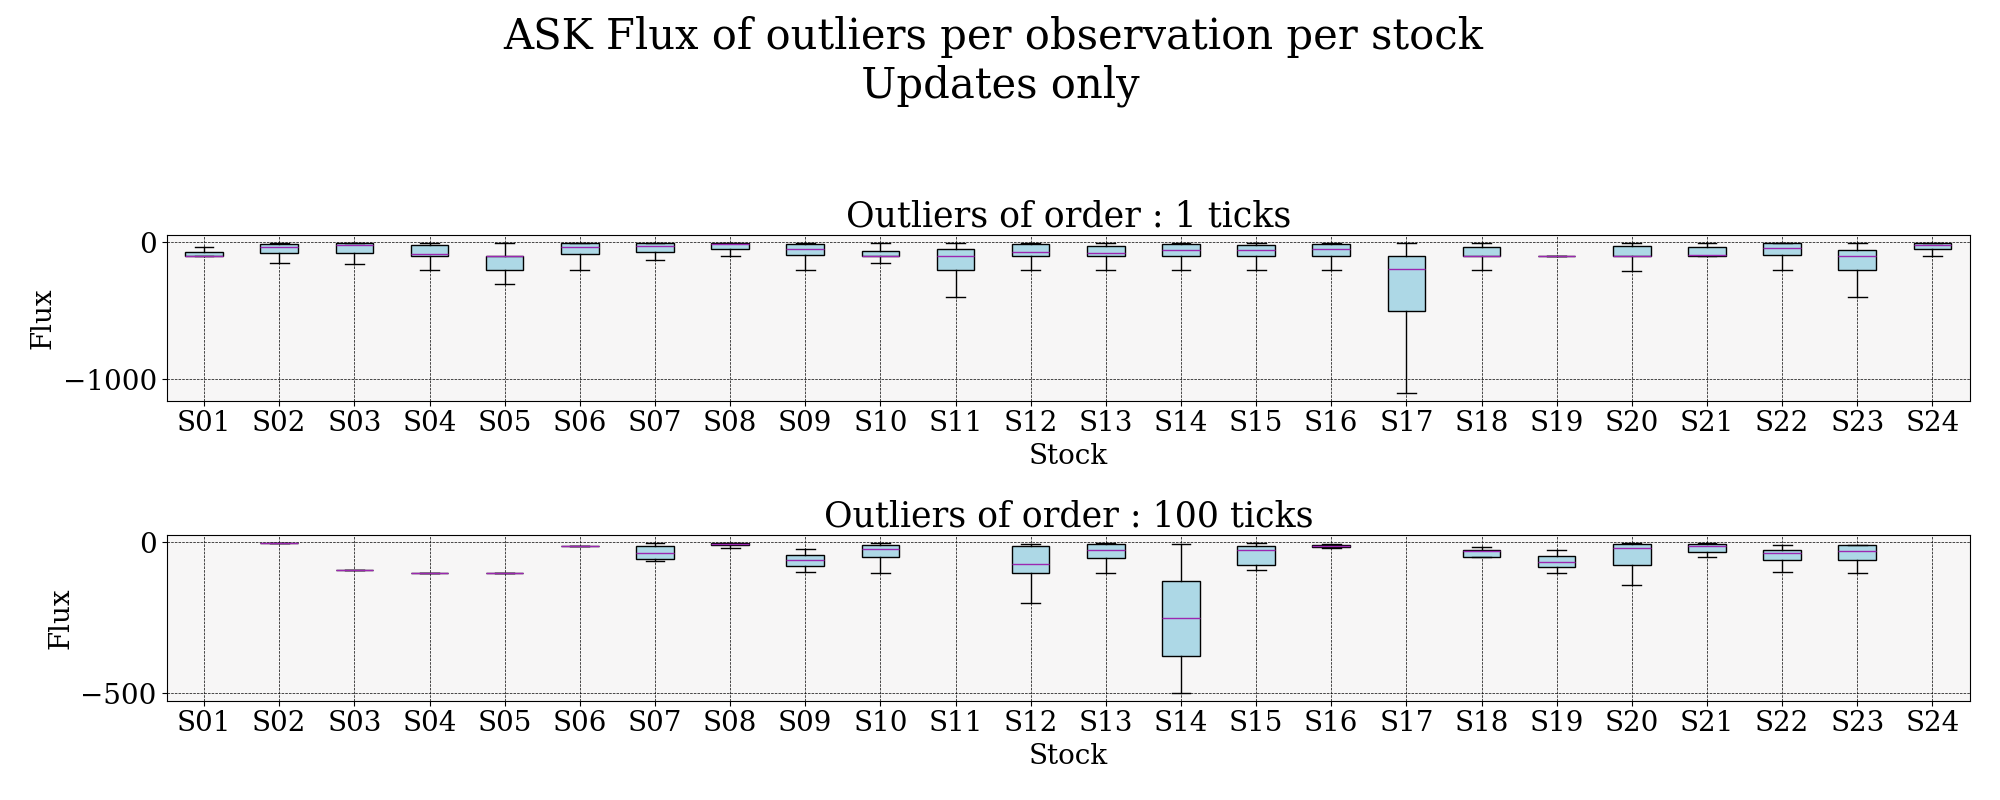
\includegraphics[width=\columnwidth]{figures/boxplot_flux_outliers_ASK_UPDATE.png}
    \caption{Boxplot of the flux of the ask price outliers for each stock. Only the ask update outliers are considered.}
    \label{fig:flux_ask_update}
\end{figure}

\begin{figure}[H]
    \centering
    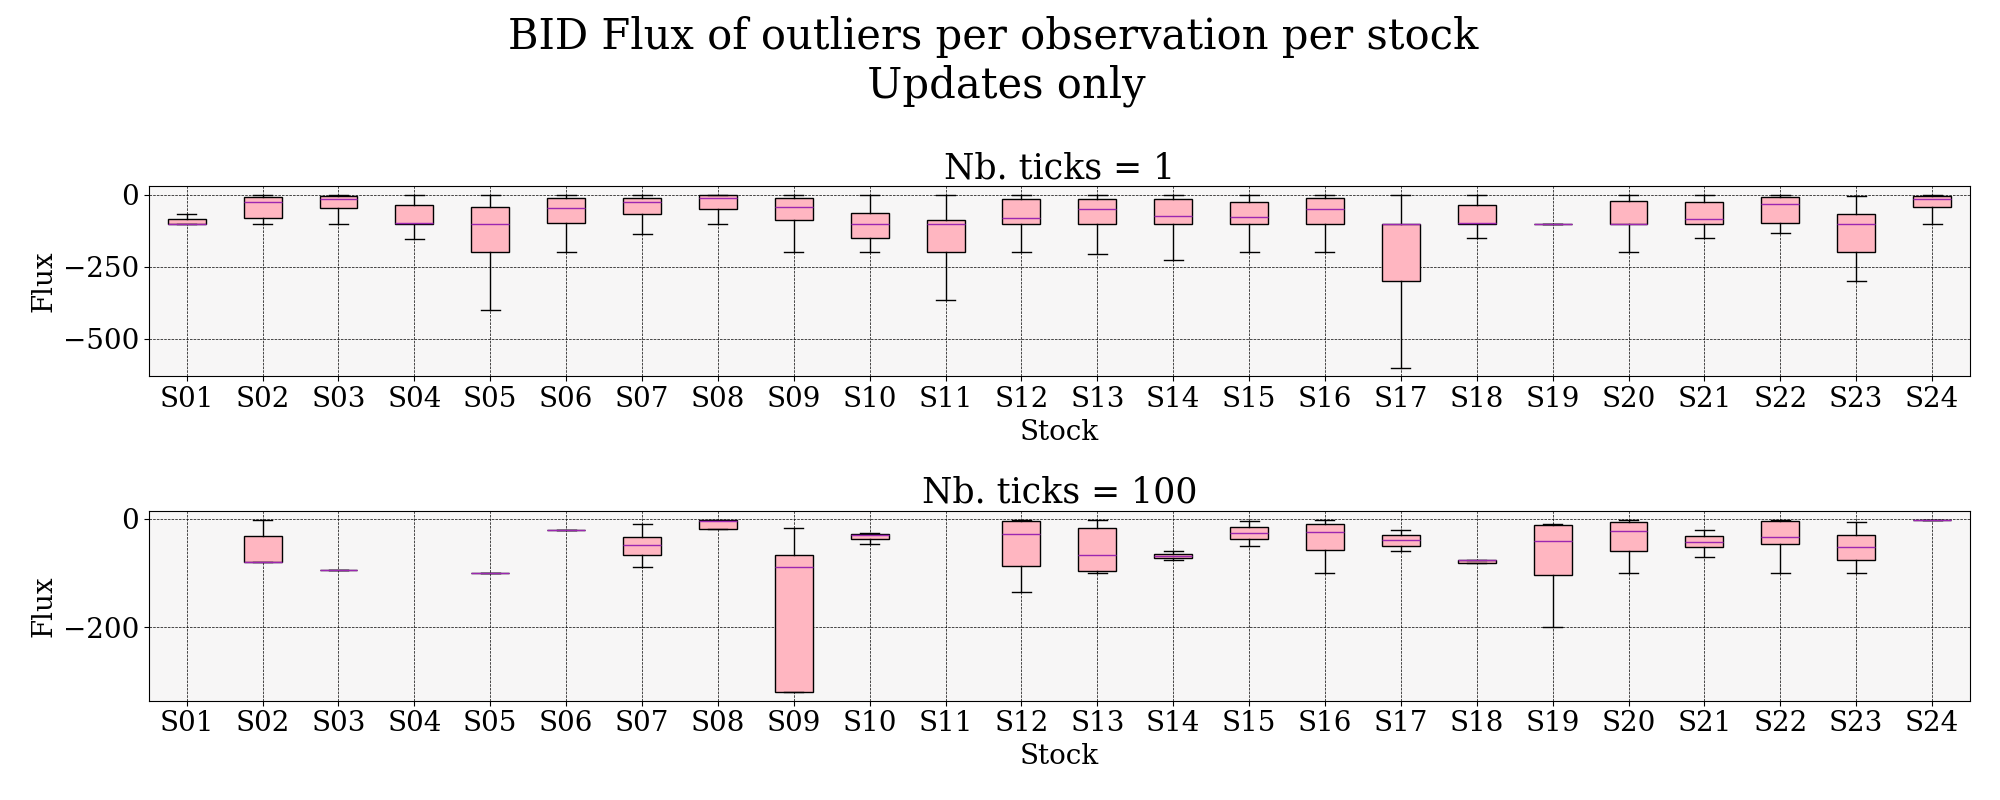
\includegraphics[width=\columnwidth]{figures/boxplot_flux_outliers_BID_UPDATE.png}
    \caption{Boxplot of the flux of the bid price outliers for each stock. Only the bid addition updates are considered.}
    \label{fig:flux_bid_update}
\end{figure}

\begin{figure}[H]
    \centering
    \begin{subfigure}{0.49\columnwidth}
        \centering
        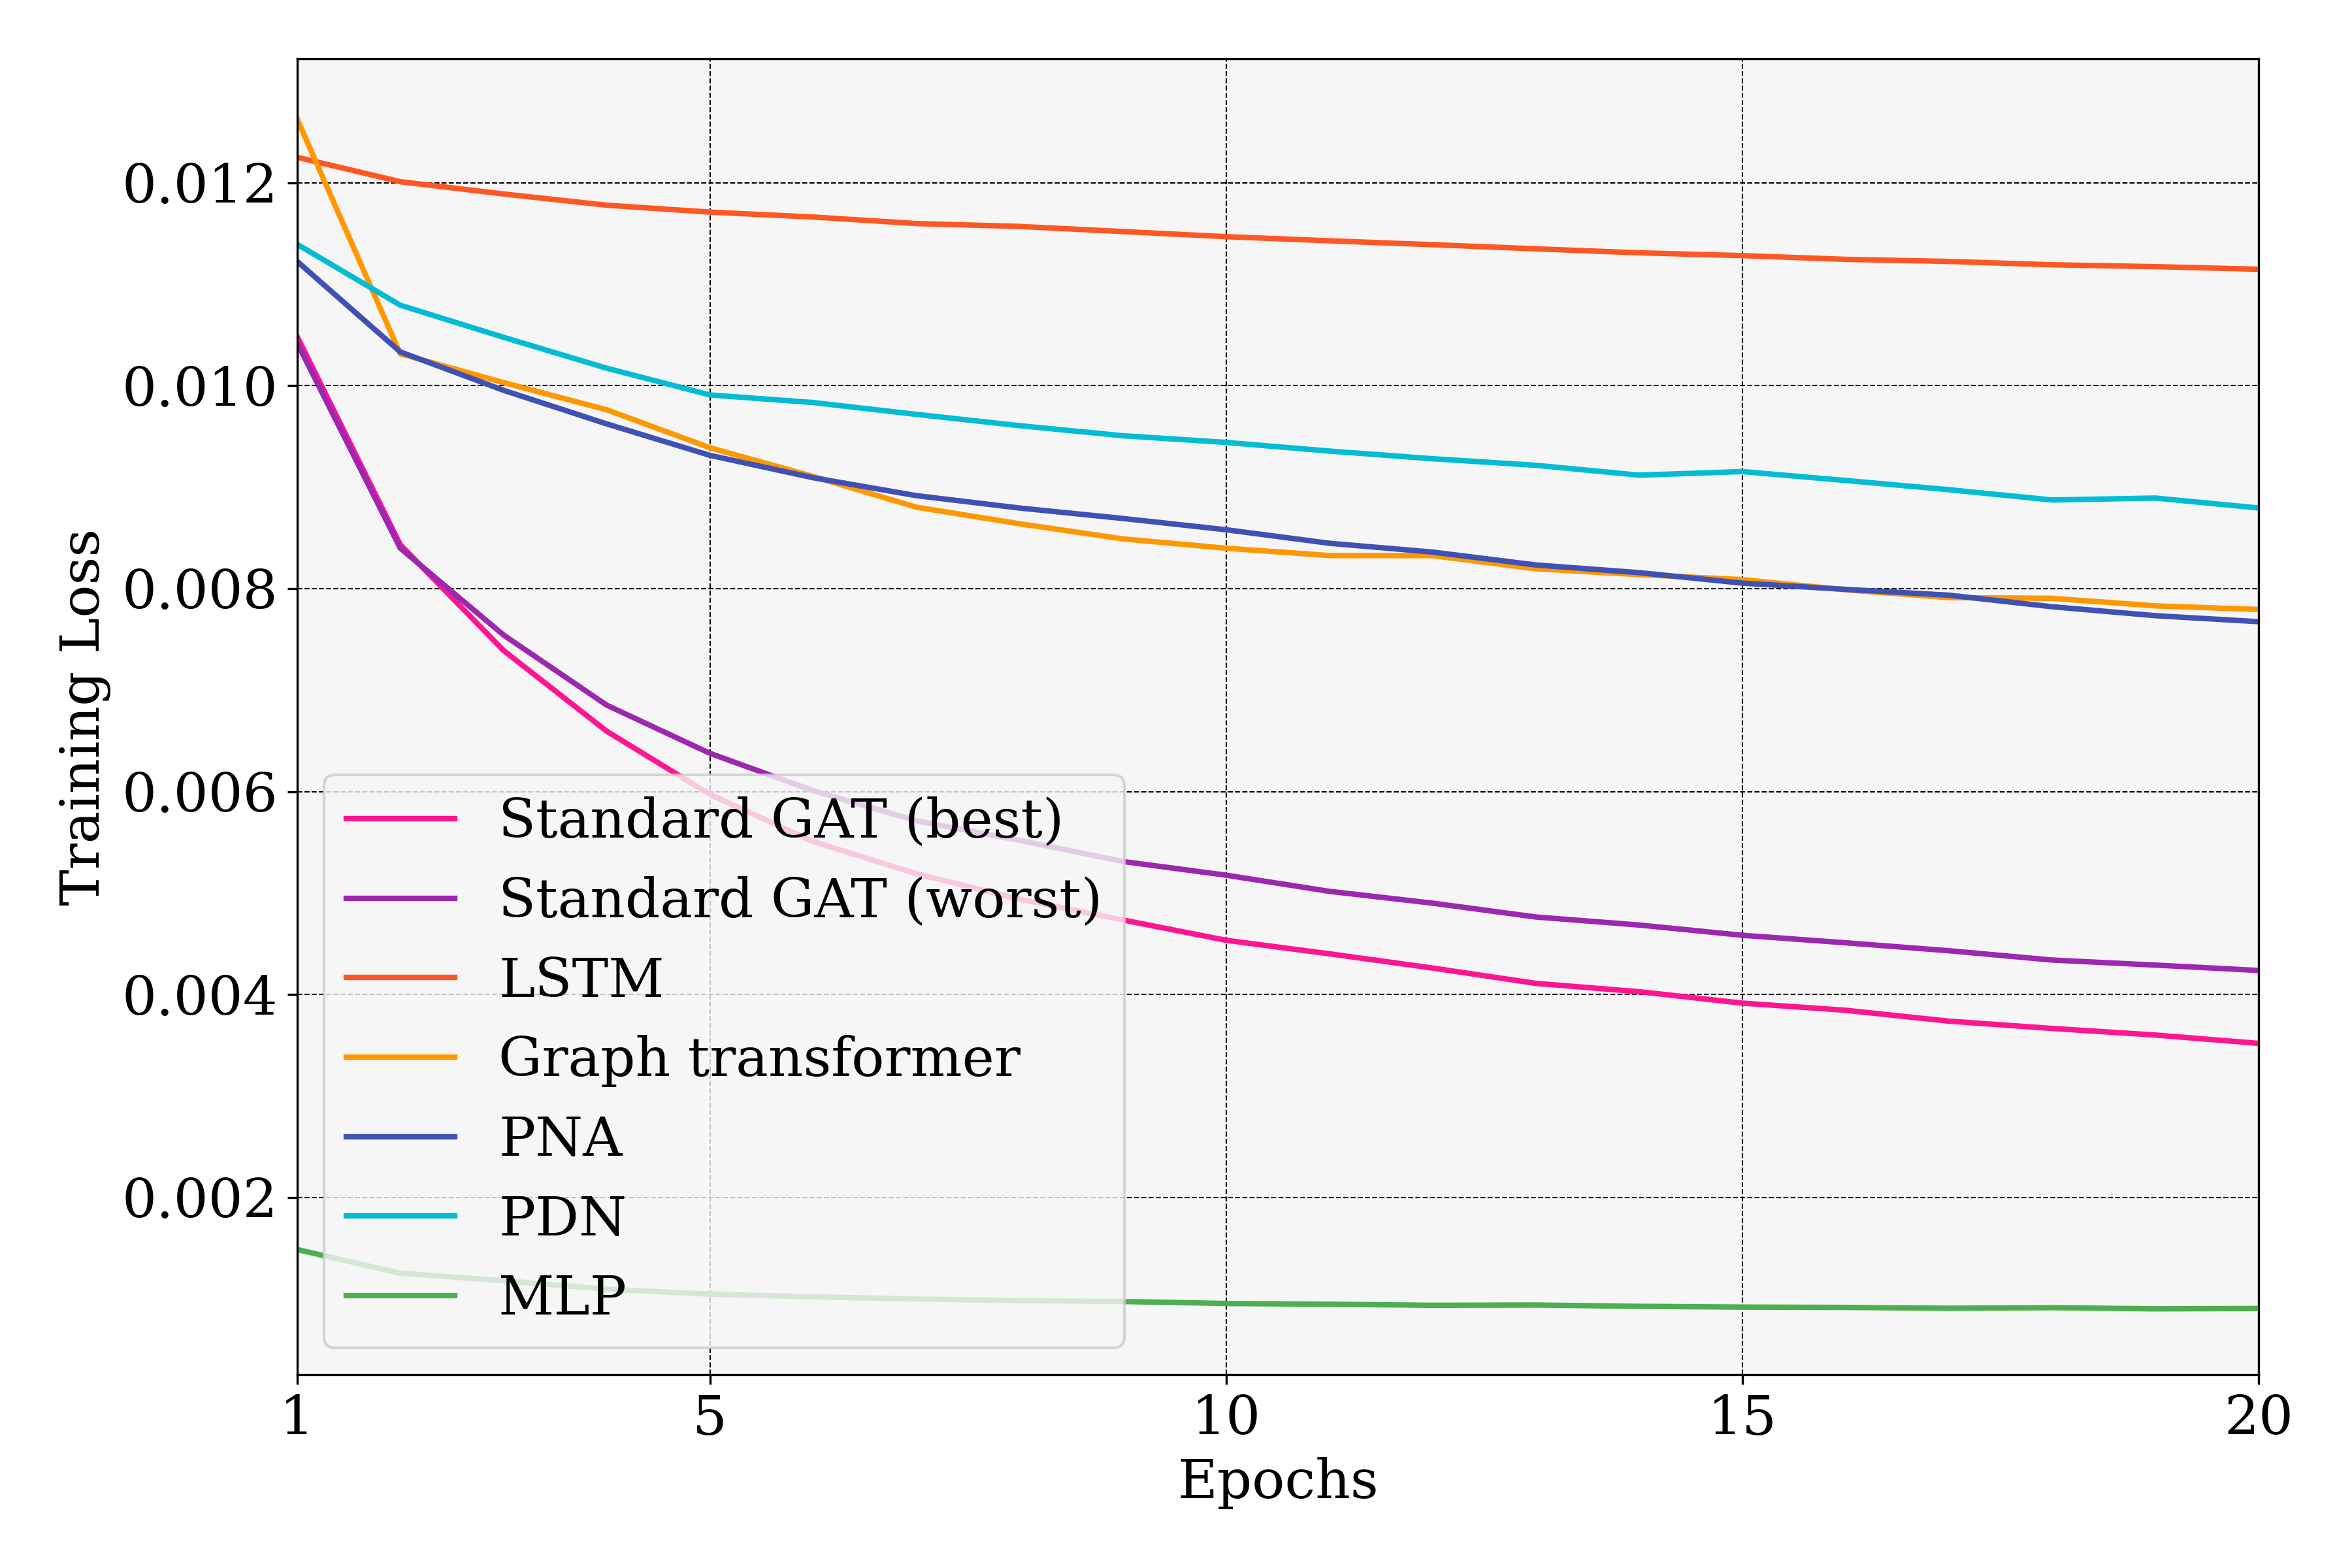
\includegraphics[width=0.99\columnwidth]{figures/train_loss.png}
        \caption{Training loss}
        \label{fig:train_loss}
    \end{subfigure}
    \begin{subfigure}{0.49\columnwidth}
        \centering
        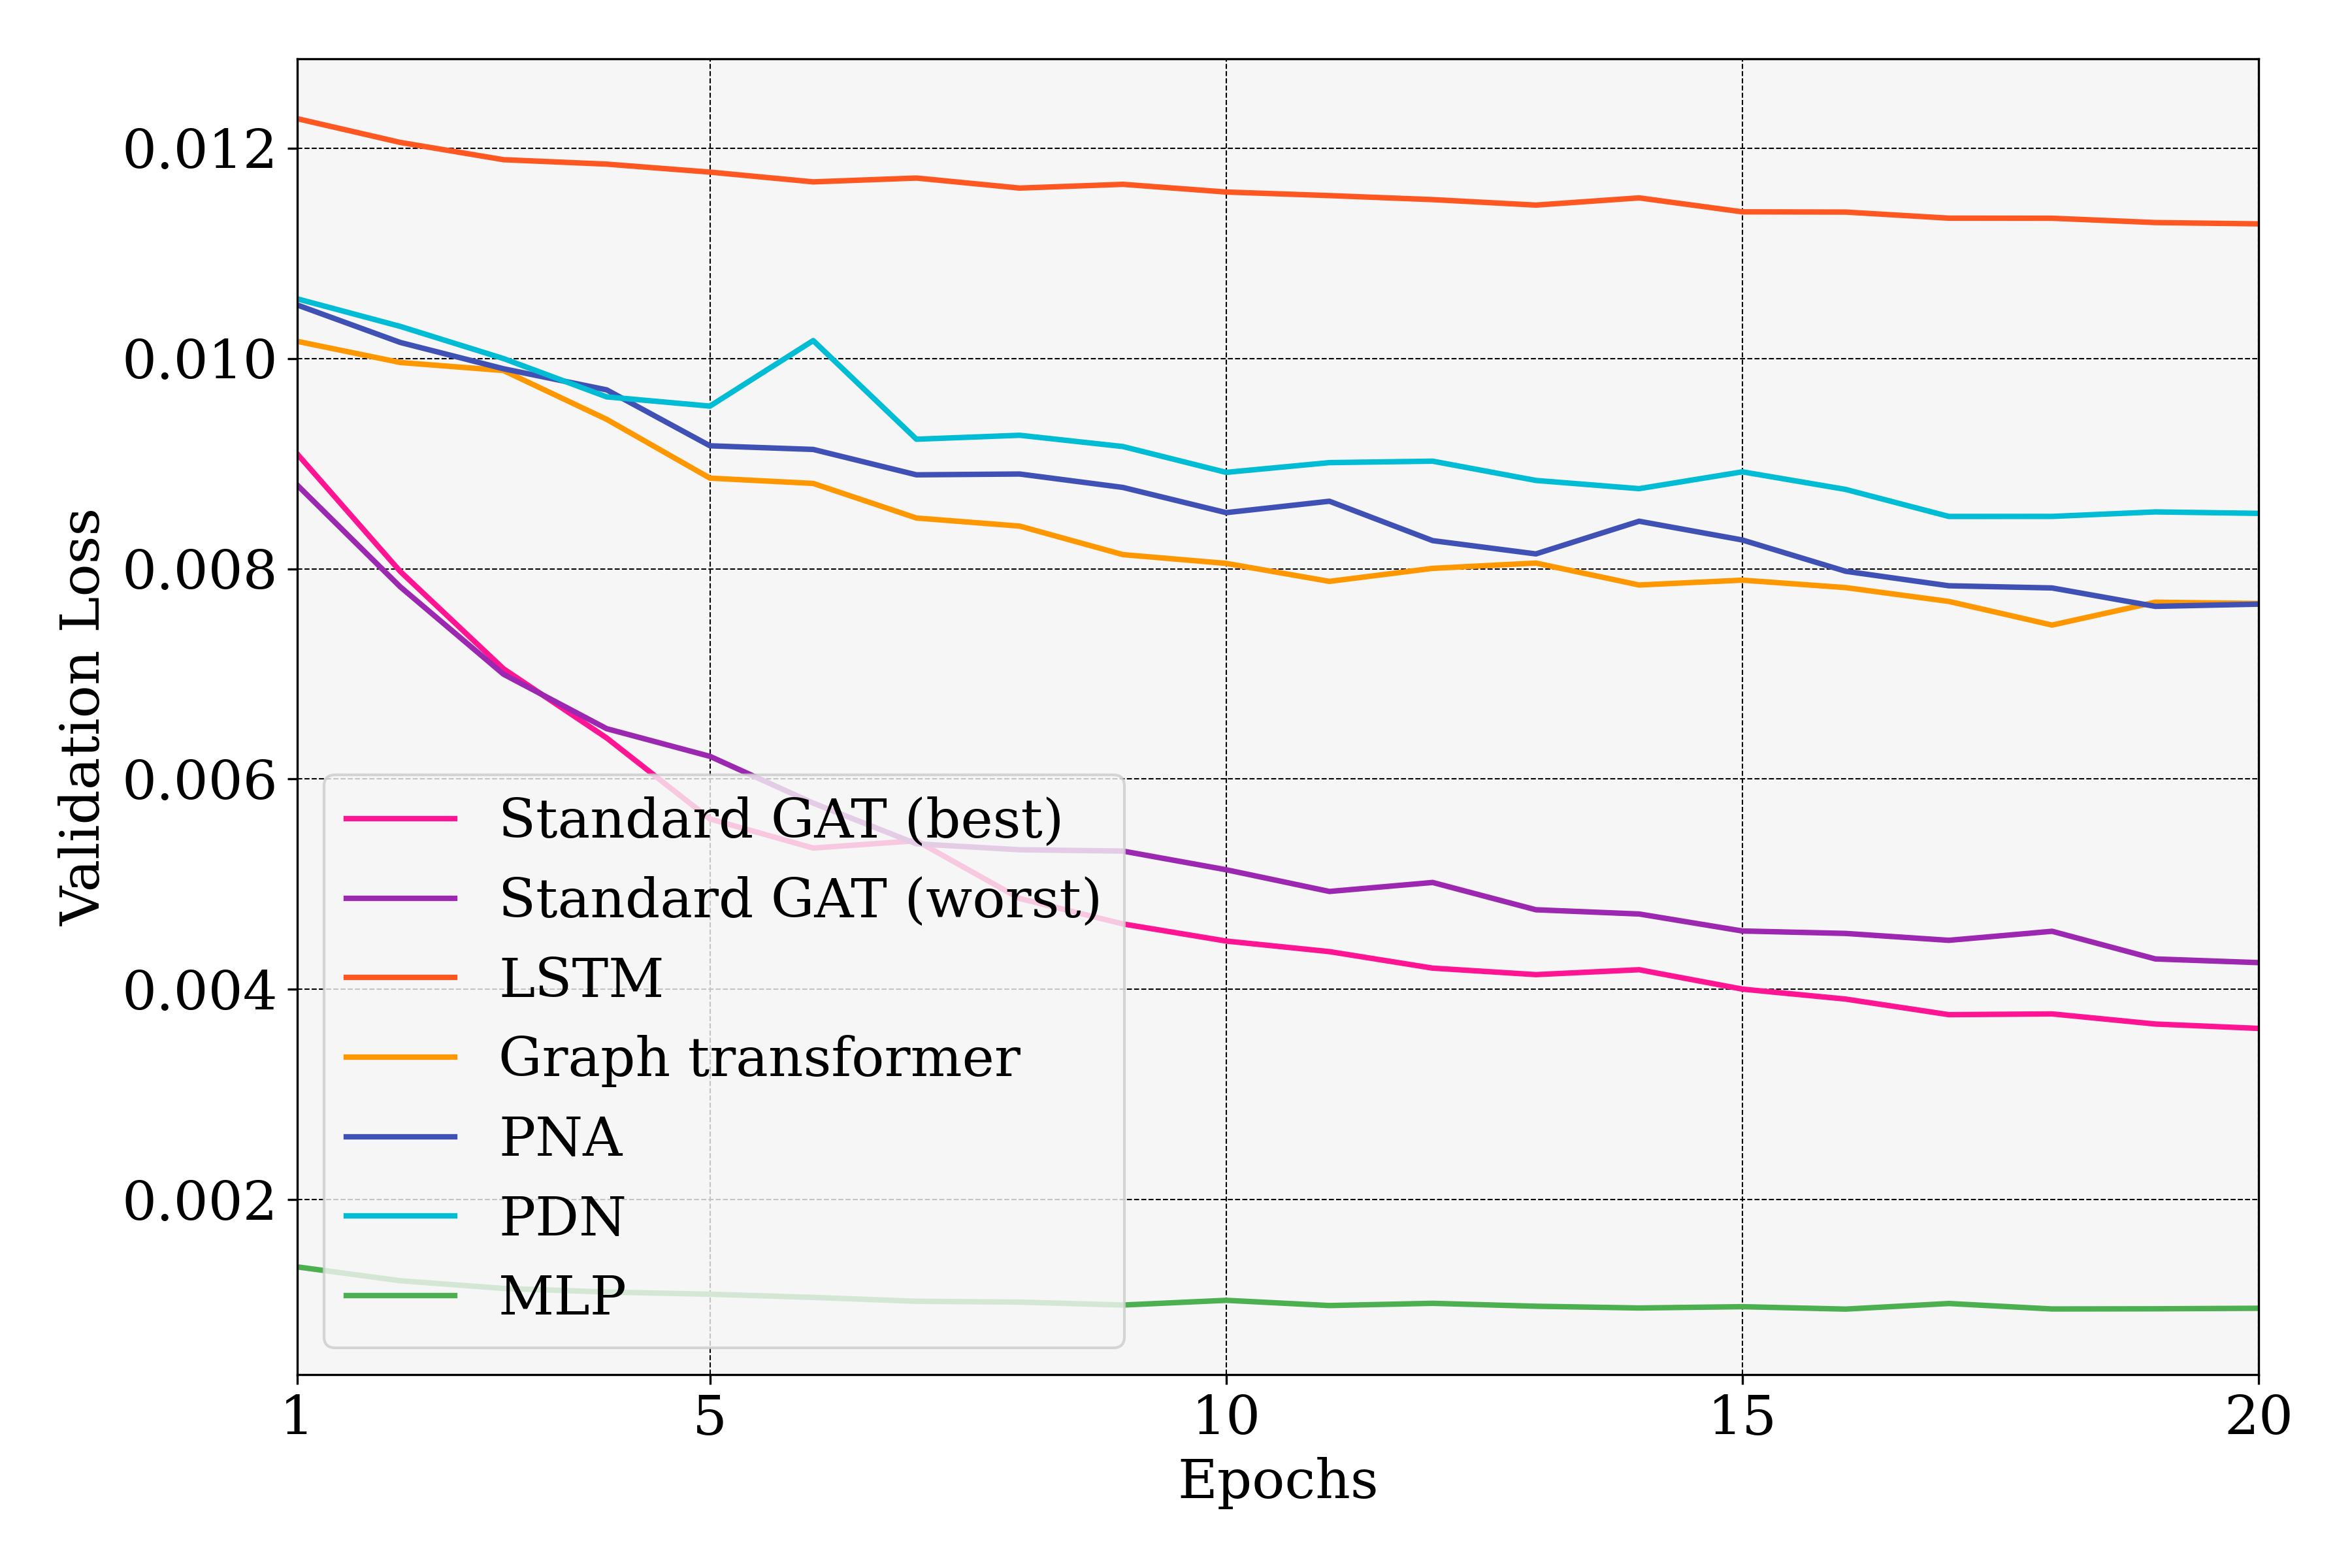
\includegraphics[width=0.99\columnwidth]{figures/val_loss.png}
        \caption{Validation loss}
        \label{fig:val_loss}
    \end{subfigure}
    \caption{Training and validation loss}
\end{figure}

\begin{figure}[H]
    \centering
    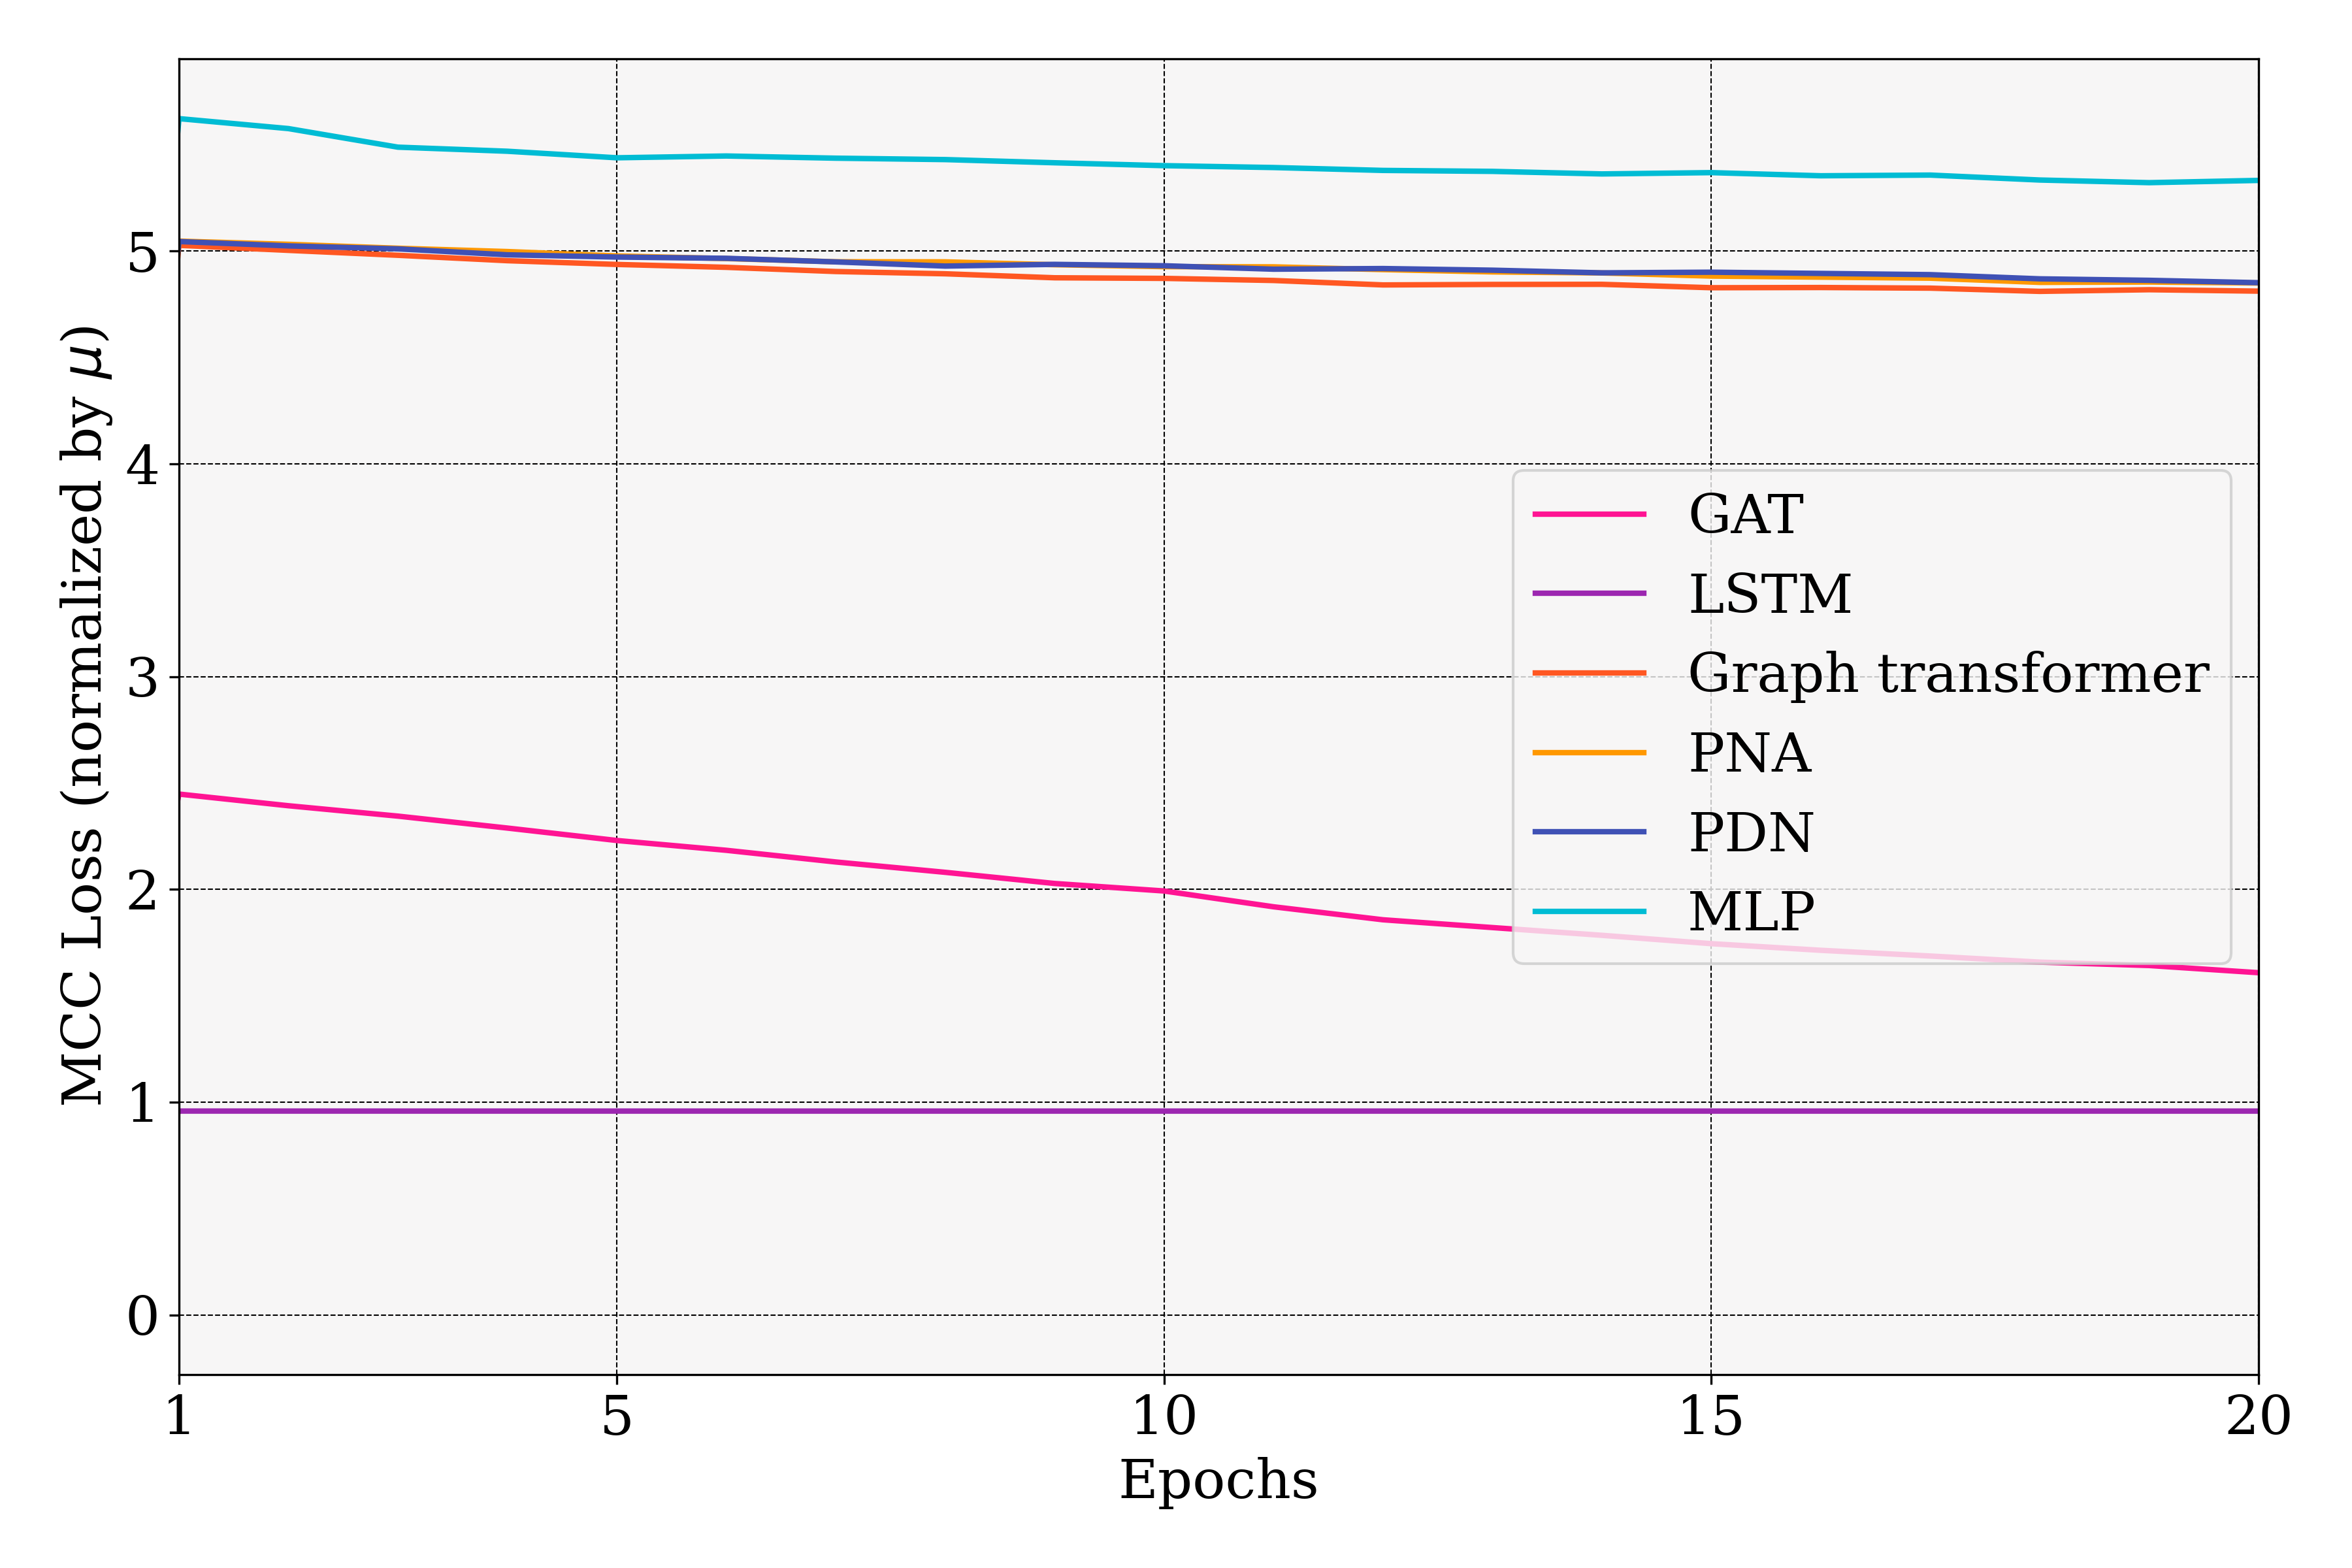
\includegraphics[width=0.5\columnwidth]{figures/mcc_loss.png}
    \caption{MCC loss on the test set}
    \label{fig:mcc_loss}
\end{figure}


\end{document}